\documentclass[a4paper,12pt]{report}
\usepackage{titlesec}
\usepackage[T1]{fontenc}
\usepackage[utf8]{inputenc}
\usepackage[french]{babel}
\usepackage{enumitem}
\usepackage{pifont}
\usepackage{graphicx}
\usepackage{chngcntr} 
\usepackage{placeins}
\usepackage{float}
\usepackage{amssymb}
\usepackage{longtable}
\usepackage{array}
\usepackage{ragged2e}
\usepackage{booktabs}
\usepackage[table]{xcolor}
\usepackage[T1]{fontenc}
\usepackage[margin=1in]{geometry}

% Core packages
\usepackage{amsmath,amssymb}
\usepackage{tikz-cd}
\usetikzlibrary{calc}
\usepackage{tikzpagenodes}
\usepackage{eso-pic}
\usepackage{multicol}
\usepackage{array}
\usepackage{float}
\usepackage{tabularx}
\usepackage{ragged2e}

\newcolumntype{Y}{>{\RaggedRight\arraybackslash}X}
\newcolumntype{C}[1]{>{\centering\arraybackslash}p{#1}}


% Paragraphs
\setlength{\parindent}{0pt}
\setlength{\parskip}{1\baselineskip}
 % décale la numérotation des sections pour qu'elle ne dépende plus du chapitre
\definecolor{rowalt}{gray}{0.95}
\newcommand{\sone}{Sprint 1}
\newcommand{\stwo}{Sprint 2}
\newcommand{\sthree}{Sprint 3}
\newcommand{\phigh}{Haute}
\newcommand{\pmid}{Moyenne}
\newcommand{\plow}{Faible}
\renewcommand{\thesection}{\arabic{section}} % sections = 1,2,3...
\renewcommand{\thesubsection}{\thesection.\arabic{subsection}} 

% Page decoration: bandeau décoratif en haut de chaque page
\AddToShipoutPictureBG*{%
  \begin{tikzpicture}[remember picture, overlay]
    \fill[gray!10] ($(current page.north west)+(1cm,-0.8cm)$) rectangle ($(current page.north east)+(-1cm,-1.5cm)$);
    \draw[line width=0.5pt] ($(current page.north west)+(1cm,-0.8cm)$) rectangle ($(current page.north east)+(-1cm,-1.5cm)$);
  \end{tikzpicture}%
}

\begin{document}
\sloppy
\pagenumbering{gobble}

\tableofcontents
\newpage

\listoftables
\addcontentsline{toc}{chapter}{Liste des tableaux}
\newpage

\listoffigures
\addcontentsline{toc}{chapter}{Liste des figures}
\newpage

\pagenumbering{arabic}
\setcounter{page}{1}
\chapter*{Introduction générale}
\addcontentsline{toc}{chapter}{Introduction générale}

Aujourd'hui, l'obésité et les maladies liées à une mauvaise hygiène de vie constituent l'un des principaux défis de santé publique au niveau mondial. Devant la sédentarité croissante et les habitudes alimentaires déséquilibrées, de plus en plus de personnes cherchent des solutions efficaces pour reprendre le contrôle de leur santé, améliorer leur condition physique et adopter un mode de vie plus sain. C'est dans ce cadre que les plateformes numériques dédiées au fitness et à la nutrition se sont imposées comme des outils essentiels, permettant aux utilisateurs de bénéficier d'un accompagnement personnalisé et accessible pour suivre leurs activités physiques, gérer leur alimentation et atteindre leurs objectifs de bien-être.



Notre projet de fin d'études en vue de l'obtention du Diplôme de Mastère professionnel en Intelligence Artificielle et Internet des Objets, s'inscrit dans cette perspective. Notre objectif est de créer UFitPal, une plateforme intelligente de fitness et de nutrition. Ce projet vise à développer une application web permettant d'offrir un suivi personnalisé aux athlètes, de faciliter la collaboration avec des coachs sportifs et des nutritionnistes, et d'intégrer des modules d'intelligence artificielle pour optimiser les recommandations et
 modéliser les comportements des utilisateurs.

Ce rapport comprend les différentes étapes et tâches que nous avons accomplies lors de la réalisation de ce projet. Il comporte quatre chapitres :

\begin{itemize}[leftmargin=*, itemsep=4pt]
    \item Dans le premier chapitre, nous abordons le cadre général du projet en présentant l'organisme d'accueil, la description et les objectifs d'UFitPal, ainsi qu'une étude de l'existant et la méthodologie de travail adoptée.
    \item Le deuxième chapitre expose les acteurs du système, ainsi que les exigences fonctionnelles et non fonctionnelles de l'application, l'architecture technique retenue, le Product Backlog global et l'environnement de développement utilisé.
    \item Le troisième chapitre vise à présenter le Sprint 1, comprenant la conception et le développement des fonctionnalités d'authentification, de gestion des profils et de communication entre les différents acteurs de la plateforme.
    \item Le quatrième chapitre est consacré au Sprint 2, dédié au suivi sportif et nutritionnel de l'athlète, à la gestion des plans repas par le nutritionniste, ainsi qu'à l'intégration des modules d'intelligence artificielle, incluant les modèles prédictifs et le chatbot IA.
\end{itemize}

Enfin, une conclusion générale et perspectives résume le travail accompli et illustre les améliorations et extensions envisageables pour la plateforme UFitPal.

\newpage

\chapter*{Chapitre 1: Présentation du projet}  % Pas de numéro ajouté automatiquement
\addcontentsline{toc}{chapter}{Chapitre 1: Présentation du projet}  % Ajoute dans le sommaire

\section{Introduction du chapitre}
Dans ce chapitre, nous présentons le cadre général de notre stage au sein de HOLMENA Company for Digital Solutions. Nous introduisons l’entreprise d’accueil, ses domaines d’activité ainsi que les services qu’elle propose. Nous décrivons ensuite le projet réalisé et ses objectifs principaux. Enfin, l’étude de l’existant permet de cerner la problématique et de démontrer la valeur ajoutée de la solution développée.

\section{Présentation de l’organisme}

HOLMENA Company for Digital Solutions est une entreprise innovante fondée en 2024, spécialisée dans les solutions informatiques et numériques au sein de la région MENA.  
HOLMENA est une équipe jeune et pleine d'énergie réunie pour satisfaire les besoins de ses clients et les soutenir tout au long de leurs projets.
\begin{figure}[htbp]
    \centering
    
\includegraphics[width=0.5\textwidth]{images/image.jpeg}
    \caption{Logo de HOLMENA Company for Digital Solutions}
    \label{fig:holm}
\end{figure}

\FloatBarrier
\subsection{L’équipe de la société}

C’est une entreprise spécialisée dans les solutions digitales, le web et l’intelligence artificielle, dirigée par une équipe fondatrice dynamique et complémentaire :

\begin{itemize}
    \item Gérant (Fondateur \& Project Manager) : Mohamed Rashad Rouine
    \item Direction Générale
    \item Direction Technique
    \item Service Opérations Digitales (Co-Founder \& Digital Operations Specialist)
    \item Direction Stratégique (Co-Founder \& Chief Strategic Officer)
    \item Service Développement \& Croissance
    \item Service Design \& Communication (Chief Designer)
\end{itemize}

\subsection{Services}

\begin{itemize}
    \item Services digitaux et intégration de solutions numériques innovantes.
    \item Services de recherche et développement en technologies IT.
    \item Services de conception Web / mobile et développement d'applications performantes.
    \item Développement de solutions e-commerce sécurisées et évolutives.
    \item Services de création de contenu multimédia et gestion de présence digitale.
\end{itemize}

\section{Présentation du projet}

\subsection{Contexte du projet}
Dans le cadre de notre projet de fin d'études en vue de l'obtention du Diplôme de Mastère professionnel en intelligence artificielle \& internet des objets, j’ai effectué un stage à l’entreprise HOLMENA Company for Digital Solutions afin de concevoir et développer une plateforme innovante intitulée UFitPal : Assistance intelligente en fitness et nutrition.

\subsection{Description du projet}
Notre projet consiste à concevoir et développer une plateforme intelligente de fitness et de nutrition, capable d'offrir une expérience personnalisée et innovante aux utilisateurs grâce à l'intelligence artificielle. Elle propose des programmes d’entraînement et des plans nutritionnels personnalisés, qui s'adaptent aux besoins spécifiques de chaque utilisateur.

\subsection{Les objectifs}
Notre objectif est de créer une plateforme pour le fitness et la nutrition qui répondra aux besoins spécifiques du public MENA. En effet, l'application offre les services suivants :

\begin{itemize}[label=\ding{51}]
  \item Mettre en place des programmes d'entraînement complètement personnalisés en fonction du niveau physique, des objectifs et du rythme de vie de l'utilisateur.
   \item Proposer des recommandations alimentaires personnalisées qui respectent les besoins énergétiques, les objectifs de santé et le mode de vie de chaque utilisateur.
  \item Offrir des interfaces simples et intuitives pour les différents profils (athlète, coach, nutritionniste).
  \item Assurer l'intégrité, la sécurité et la cohérence des données à chaque mise à jour et insertion.
  \end{itemize}
\section{Étude de l’existant du projet}
L'analyse de l'existant se divise principalement en trois parties : la description de l'existant, la critique de l'existant et la solution suggérée.
\subsection{Description de l’existant du projet}
L'objectif de cette partie est d'examiner les solutions existantes dans le domaine 
des applications de fitness et nutrition afin de mieux cerner les besoins spécifiques du projet UFitPal, 
et de les intégrer de manière intelligente dans sa conception et son développement.

Nous avons donc examiné les applications les plus populaires disponibles à l'échelle mondiale et dans la région MENA.

Nous citons :

\begin{itemize}

\item \textbf{ArabFit} est une application mobile de fitness arabophone, disponible sur iOS et Android, 
destinée aux utilisateurs du Maghreb et de la région MENA. Elle est conçue pour aider les utilisateurs 
à développer leur musculature, perdre du poids et obtenir les meilleurs résultats grâce à des exercices 
physiques quotidiens.

\begin{figure}[H]
    \centering
    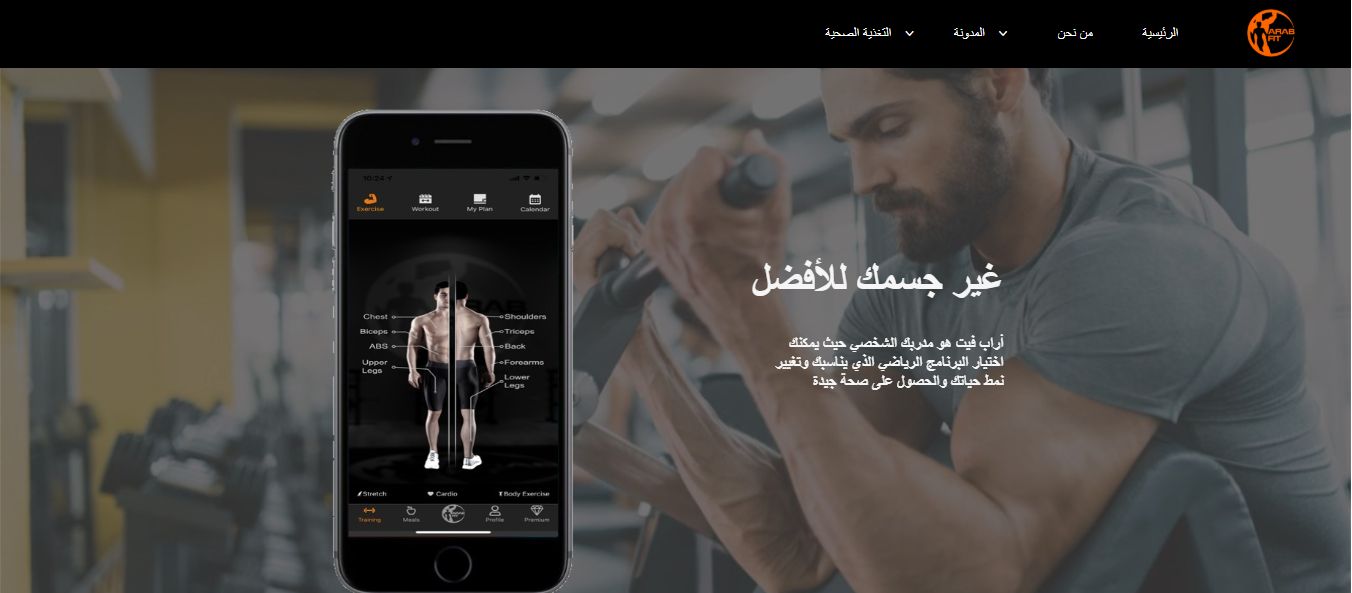
\includegraphics[width=1\textwidth]{images/arbfit.png}
    \caption{Interface de l'application ArabFit}
    \label{fig:arbfit}
    
\end{figure}

\FloatBarrier


\item \textbf{MyFitnessPal} est une application américaine de suivi nutritionnel et sportif, 
lancée en 2005 et rachetée par Under Armour en 2015. 

\begin{figure}[H]
    \centering
    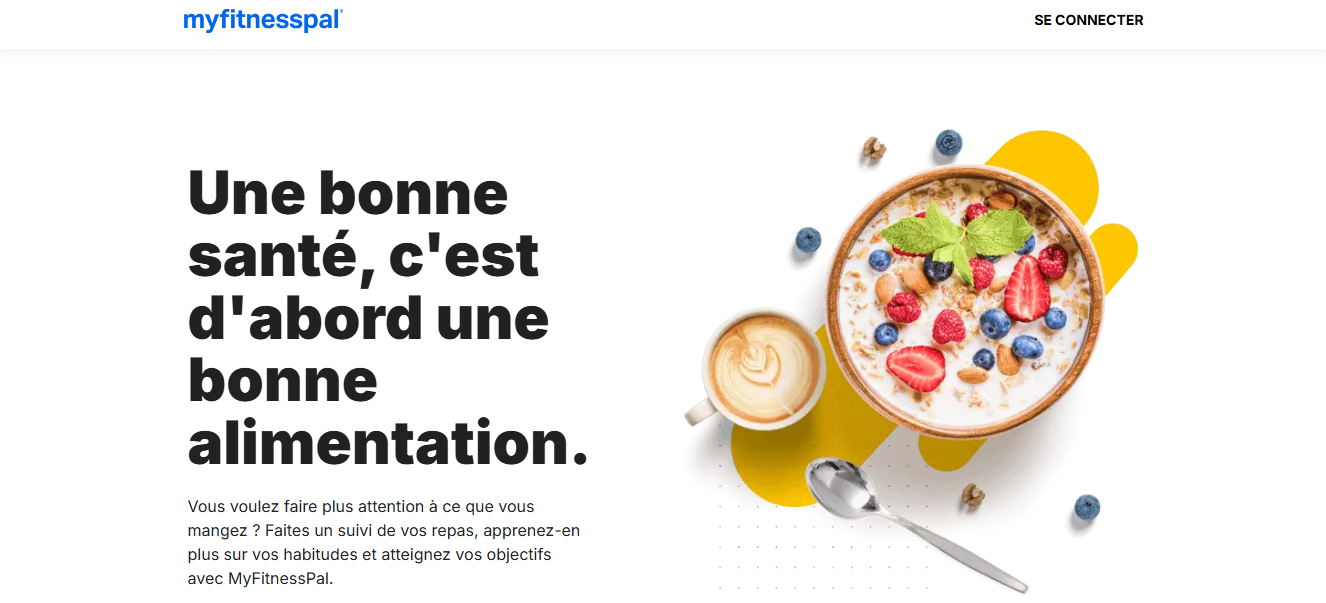
\includegraphics[width=1\textwidth]{images/myfitt.png}
    \caption{Interface de l'application MyFitnessPal}
    \label{fig:myfitnesspal}
    
\end{figure}
\vspace{-1cm} 
\FloatBarrier

\end{itemize}

\subsection{Problématique}
Comment concevoir et implémenter une plateforme numérique de santé préventive et intelligente qui unifie l'accompagnement humain (coachs et nutritionnistes), 
l'analyse métabolique et l'intelligence artificielle prédictive, afin d'offrir des recommandations ultra-personnalisées, de détecter de manière proactive les stagnations
 physiques et de maximiser l'adhésion à long terme des utilisateurs ? 

 
  
 
\subsection{Critique de l'existant}

L'objectif de cette étape est d'identifier les principales anomalies observées, 
pour analyser les causes profondes et trouver des solutions adaptées.
Dans notre étude, nous avons observé les éléments suivants :

\begin{itemize}[label=$\star$]
 \item  Personnalisation limitée, reposant sur des paramètres statiques (âge, poids, objectif calorique),
 sans moteur d'IA adaptatif capable d'évoluer en fonction des progrès de l'utilisateur.
 \item Aucun suivi nutritionnel n'est autorisé, sauf dans le cas d'une journalisation descriptive, 
 sans analyse intelligente ni recommandations personnalisées.
 \item Aucune dimension de relation professionnelle n'est intégrée : pas d'espace dédié à la relation athlète-coach ou athlète-nutritionniste, 
 ni de messagerie structurée, ni de module de planification de rendez-vous.
 \item Ces solutions ne contiennent aucune fonctionnalité d'intelligence artificielle avancée, telle que la prédiction d'évolution,
 la détection de plateau sportif ou un assistant de conseils personnalisés.
 \item Le suivi corporel est partiel, centré principalement sur le poids et les calories, sans intégration des métriques
 anthropométriques ni outils de visualisation de la progression.
 \end{itemize}
  


\subsection{Les solutions proposées}
Face aux défis identifiés dans l'étude de la situation existante,
 notamment la fragmentation des données et le manque d'adaptation aux spécificités de la région MENA,
  nous proposons une solution innovante baptisée UFitPal:

\begin{itemize}[label=$\star$]
\item  Mise en place de programmes sportifs et nutritionnels personnalisés en fonction du profil utilisateur (âge, objectifs, contraintes), 
grâce à un système d'intelligence artificielle adaptatif.

\item  Un espace professionnel dédié permettant au coach et au nutritionniste d'envoyer des invitations, de gérer leurs athlètes, 
de rédiger des notes de suivi, de créer des plans repas personnalisés et de planifier des rendez-vous .
\item Évaluation prédictive des performances grâce à des modèles de machine learning : score de risque d'abandon, prédiction d'évolution du poids, 
probabilité d'atteinte de l'objectif fitness et détection automatique des plateaux sportifs.
\item Un assistant chatbot IA disponible pour l'athlète afin d'obtenir des conseils personnalisés sur la nutrition et l'entraînement.
 \item Une interface ergonomique, intuitive et multilingue qui regroupe toutes les données pour éviter la dispersion et encourager l'adhésion à long terme.
\end{itemize}

\section{Méthodologie de travail}

\subsection{Choix d'une approche agile}
Pour le développement de l'application UFitPal, nous avons adopté une méthodologie agile afin de
 répondre aux exigences évolutives d'un projet numérique innovant. Les approches agiles, contrairement 
 aux approches traditionnelles en cascade, favorisent des cycles de développement courts et itératifs 
 qui permettent une adaptation rapide aux retours des utilisateurs et aux contraintes techniques rencontrées tout au long du projet.

\subsection{Méthodologie adoptée : Scrum}
Parmi les cadres agiles disponibles, nous avons choisi Scrum pour sa structure bien définie et sa capacité à organiser efficacement le travail en équipe.
 Dans le cadre du projet UFitPal, cette méthodologie nous a permis de livrer des incréments fonctionnels à chaque sprint,
  tout en conservant une vision globale du produit final.

\subsubsection{Organisation de l'équipe}
L'équipe projet a été structurée selon les rôles Scrum suivants :
\begin{itemize}
    \item \textbf{Product Owner} : chargé de recueillir les besoins des utilisateurs cibles 
    (sportifs, coachs) et de prioriser les fonctionnalités du backlog en fonction de leur 
    valeur métier.
    \item \textbf{Scrum Master} : responsable du respect du cadre Scrum, de la levée des 
    obstacles et de la fluidité des cérémonies.
    \item \textbf{Équipe de développement} : constituée de développeurs front-end et back-end, 
    d'un designer UI/UX et d'un spécialiste en intelligence artificielle, assurant la 
    réalisation technique des fonctionnalités définies.
\end{itemize}

\subsubsection{Artefacts utilisés}
Les artefacts Scrum suivants ont structuré notre gestion du projet :
\begin{itemize}
    \item \textbf{Product Backlog} : liste vivante et priorisée de l'ensemble des 
    fonctionnalités d'UFitPal, alimentée en continu par les retours utilisateurs et les 
    évolutions des besoins.
    \item \textbf{Sprint Backlog} : sous-ensemble du Product Backlog sélectionné à chaque 
    début de sprint, découpé en tâches assignées aux membres de l'équipe.
    \item \textbf{Incrément} : version fonctionnelle et testable de l'application livrée 
    à l'issue de chaque sprint, enrichissant progressivement les fonctionnalités de la 
    plateforme.
\end{itemize}

\subsubsection{Cérémonies pratiquées}
Afin d'assurer un suivi régulier et une communication efficace au sein de l'équipe, nous 
avons mis en place les cérémonies Scrum suivantes :
\begin{itemize}
    \item \textbf{Sprint Planning} : tenue en début de chaque sprint pour définir les 
    objectifs à atteindre et répartir les tâches entre les membres de l'équipe.
    \item \textbf{Daily Scrum} : point quotidien de quinze minutes permettant à chaque 
    membre de partager son avancement, ses blocages et ses objectifs du jour.
    \item \textbf{Sprint Review} : présentation de l'incrément réalisé aux parties 
    prenantes afin de valider les fonctionnalités développées et d'ajuster les priorités.
    \item \textbf{Sprint Retrospective} : réunion d'équipe visant à analyser le déroulement 
    du sprint écoulé, à capitaliser sur les bonnes pratiques et à corriger les 
    dysfonctionnements identifiés.
\end{itemize}

\subsection{Organisation en sprints}
Le projet UFitPal a été découpé en sprints d'une durée de deux semaines chacun. Cette 
cadence nous a permis de maintenir un rythme de livraison régulier tout en intégrant 
progressivement les fonctionnalités clés de l'application, depuis la gestion des profils 
utilisateurs jusqu'à l'intégration du module d'intelligence artificielle. Le détail des 
sprints réalisés et de leurs livrables est présenté dans la section suivante.


\section{Conclusion }
Ce chapitre a présenté une perspective globale de la société d'accueil, analysé des applications 
existantes aux fonctionnalités similaires à celles que nous voulons développer, et exposé la 
méthodologie de travail adoptée.Dans le prochain chapitre, nous procédons à la 
spécification des besoins fonctionnels et non-fonctionnels, à la définition de l'architecture 
technique de l'application, ainsi qu'à la présentation du Product Backlog global et de 
l'environnement de travail retenu.

\chapter*{Chapitre 2 : Réalisation de l'Application}
\addcontentsline{toc}{chapter}{Chapitre 2 : Réalisation de l'Application}

\setcounter{section}{0}
\section{Introduction du chapitre}
Ce chapitre traite de la spécification des besoins du projet UFitPal, une étape cruciale pour s'assurer 
que les objectifs de la plateforme correspondent aux attentes des utilisateurs.
 Il comporte l'analyse des besoins fonctionnels et non fonctionnels, le diagramme global des cas d'utilisation, 
 l'architecture de l'application, le Product Backlog général et l'environnement de travail adopté. 
 Ces différents éléments constituent une vision claire et structurée du projet, 
 et offrent donc une base solide pour sa conception, son développement et son évolution future.
 \section{ Analyse des besoins}

 \subsection{Identification des acteurs du système}

\begin{itemize}
    \item \textbf{Visiteur} : Toute personne non authentifiée souhaitant accéder à l'application. 
    Il peut s'inscrire, se connecter via Google ou réinitialiser son mot de passe. 
    Il n'a accès à aucune fonctionnalité métier avant authentification.

    \item \textbf{Athlète} :Acteur central du système. Une fois connecté, il bénéficie de l’ensemble des fonctionnalités personnalisées :
     gestion du profil, onboarding, suivi des activités sportives, de la progression et de la nutrition, 
     consultation des résultats des modèles IA (churn, poids, objectif et plateau), 
     consultation des recommandations basées sur des règles métier, consultation du plan repas élaboré par le nutritionniste,
      interaction avec le chatbot, gestion des invitations, envoi et réception de messages avec les autres acteurs connectés.

    \item \textbf{Coach} : Professionnel de l'entraînement sportif. Il gère son profil, 
    crée et consulte des notes de suivi sur ses Athlètes, communique via la messagerie interne, 
    propose des rendez-vous et envoie des invitations aux Athlètes qu'il accompagne.

    \item \textbf{Nutritionniste} : Professionnel de la nutrition. Il gère son profil, 
    élabore des plans repas personnalisés pour ses Athlètes clients, communique via la 
    messagerie interne, et peut proposer des rendez-vous et envoyer des invitations.

   
\end{itemize}

\subsection{Spécification des besoins fonctionnels}

Cette partie est consacrée à l'énumération des besoins fonctionnels pris en charge par les 
acteurs identifiés, afin d'atteindre les fonctionnalités et objectifs du système.

\subsubsection*{Le Visiteur peut :}
\begin{itemize}
    \item \textbf{S'inscrire} : Le Visiteur peut créer un compte en fournissant les informations 
    de base (nom, email, mot de passe) et en choisissant son rôle (Athlète, Coach ou Nutritionniste).
    \item \textbf{Se connecter via Google} : Le Visiteur peut s'authentifier rapidement en 
    utilisant son compte Google, sans saisie manuelle de ses identifiants.
    \item \textbf{Réinitialiser son mot de passe} : Le Visiteur peut réinitialiser son mot de 
    passe en renseignant son adresse email afin de recevoir un lien de réinitialisation.
\end{itemize}

\subsubsection*{L'Athlète peut :}
\begin{itemize}
    \item \textbf{Gérer son profil} : L'Athlète peut consulter et mettre à jour ses informations 
    personnelles avec des champs adaptés à son rôle (âge, taille, poids, objectifs sportifs).
    \item \textbf{Gérer l'onboarding} : L'Athlète remplit un questionnaire initial portant sur 
    ses objectifs, son niveau sportif et ses préférences, afin de personnaliser son expérience 
    sur la plateforme.
    \item \textbf{Envoyer et recevoir des messages} : L'Athlète peut communiquer avec son Coach 
    et son Nutritionniste via la messagerie interne de l'application.
    \item \textbf{Ajouter ses activités sportives} : L'Athlète saisit ses séances d'entraînement 
    en précisant le type d'activité, la durée et l'intensité. Ces données alimentent les modèles 
    de machine learning.
    \item \textbf{Ajouter sa progression} : L'Athlète enregistre régulièrement ses données 
    corporelles (poids, mensurations) et ses performances afin de suivre son évolution dans 
    le temps.
    \item \textbf{Ajouter son journal alimentaire} : L'Athlète consigne ses repas quotidiens 
    dans son journal nutritionnel personnel pour assurer un suivi alimentaire complet.
    \item \textbf{Consulter le plan repas du Nutritionniste} : L'Athlète peut accéder au plan 
    repas personnalisé élaboré et assigné par son Nutritionniste.
    \item \textbf{Voir les résultats des modèles IA} : L'Athlète consulte les prédictions 
    générées par les quatre modèles de machine learning, à savoir la prédiction du churn, 
    du poids futur, de l'atteinte de l'objectif et du plateau de progression.
    \item \textbf{Consulter les recommandations} :  L'Athlète consulte ses recommandations personnalisées de nutrition (calories, macronutriments cibles) et d'entraînement (planning hebdomadaire), calculées selon ses données physiologiques, 
    afin d'optimiser sa progression en toute sécurité.
    \item \textbf{Interagir avec le chatbot IA} : L'Athlète peut dialoguer avec le chatbot 
    conversationnel  pour obtenir des conseils personnalisés 
    en temps réel.
    \item \textbf{Accepter ou refuser un rendez-vous} : L'Athlète répond aux propositions de 
    créneaux soumises par son Coach ou son Nutritionniste.
    \item \textbf{Accepter ou refuser une invitation} : L'Athlète peut accepter ou décliner 
    les invitations reçues de la part de son Coach ou de son Nutritionniste.
    
\end{itemize}

\subsubsection*{Le Coach peut :}
\begin{itemize}
    \item \textbf{Gérer son profil} : Le Coach peut consulter et mettre à jour ses informations 
    professionnelles avec des champs adaptés à son rôle (spécialité, expérience, certifications).
    \item \textbf{Gérer ses notes de suivi} : Le Coach crée, modifie et consulte ses notes 
    personnelles de suivi pour chaque Athlète dont il assure l'encadrement.
    \item \textbf{Envoyer et recevoir des messages} : Le Coach peut communiquer avec ses Athlètes 
     via la messagerie interne de l'application.
    \item \textbf{Proposer un rendez-vous} : Le Coach soumet une proposition de créneau à 
    l'Athlète concerné pour planifier une séance ou un suivi.
    \item \textbf{Gérer les invitations} : Le Coach peut envoyer des invitations à ses Athlètes 
    pour les intégrer à son suivi sur la plateforme.
\end{itemize}

\subsubsection*{Le Nutritionniste peut :}
\begin{itemize}
    \item \textbf{Gérer son profil} : Le Nutritionniste peut consulter et mettre à jour ses 
    informations professionnelles avec des champs adaptés à son rôle (spécialités nutritionnelles, 
    diplômes).
    \item \textbf{Envoyer et recevoir des messages} : Le Nutritionniste peut communiquer avec 
    ses Athlètes clients  via la messagerie interne de l'application.
    \item \textbf{Ajouter un repas personnalisé} : Le Nutritionniste crée et assigne un plan 
    repas personnalisé à l'Athlète client.
    \item \textbf{Proposer un rendez-vous} : Le Nutritionniste soumet une proposition de créneau 
    à l'Athlète concerné pour planifier un suivi nutritionnel.
    \item \textbf{Gérer les invitations} : Le Nutritionniste peut envoyer des invitations à ses 
    Athlètes clients pour les intégrer à son suivi nutritionnel sur la plateforme.
\end{itemize}

\subsection{Spécification des besoins non fonctionnels}
Ces besoins décrivent toutes les contraintes auxquelles est soumis le système pour sa réalisation et son bon fonctionnement:

\begin{itemize}
    \item \textbf{L'ergonomie des interfaces} : doit être conviviale et facile à utiliser. 
    Aucune connaissance approfondie n'est requise pour manipuler l'interface.
    \item \textbf{Sécurité } :Il est crucial de garantir la sécurité de la solution pour protéger les informations des utilisateurs.
   \item \textbf{Performance } :L'application doit être avant tout performante. Le système doit réagir rapidement, 
    quelle que soit l'action de l'utilisateur : l'accès, le chargement, et le rafraîchissement des données doit être en temps réel, souple, et rapide. 
   
    \item \textbf{Evolution } :Tout évolue, y compris les services. Doit savoir écouter les besoins de ses utilisateurs, prendre en compte leurs demandes,
     pour améliorer ses services, tout en gardant à l'esprit l'utilité et l'efficacité.
     \item \textbf{Fiabilité} : Le système doit être disponible et fonctionnel à tout moment pour l'utilisateur et Les informations doivent être mises à jour régulièrement.
\end{itemize}
\section{Diagramme général des cas d'utilisation}
Le modèle global des cas d'utilisation aide à organiser les exigences et les buts associés à un système. La figure  dépeint les scénarios 
d'utilisation fondamentaux pour obtenir une perspective globale du fonctionnement de l'application.

 \section{Architecture de l'application}
 Dans cette section, nous présentons l’architecture choisie pour notre application, en précisant les choix technologiques, le modèle d’organisation, ainsi que les relations entre les modules. 
 Cette structuration permettra de guider efficacement les phases de développement tout en assurant la cohérence du système avec les objectifs initiaux du projet.
 \subsection{Architecture physique}
 L'architecture à trois niveaux consacre une structure d'application logicielle bien établie regroupant les applications en trois niveaux informatiques tant logiques que physiques : 
 le niveau Présentation (également appelé interface utilisateur), 
 le niveau Application, qui s'occupe du traitement des données, et le niveau Données, dédié au stockage et à la gestion des données liées à l'application. 
 De plus, le modèle à trois niveaux favorise une meilleure sécurité en restreignant l’accès aux données de l'interface utilisateur, ce qui peut aider à sécuriser des informations sensibles. Globalement, cette structure propose une stratégie plus modulaire,facilitant le traitement des systèmes complexes et favorisant la croissance et les transformations de manière plus efficace qu'un modèle dual plus simpliste.

\begin{figure}[H]
    \centering
    \IfFileExists{images/architecture_application.png}{%
        \includegraphics[width=0.85\textwidth]{images/architecture_application.png}%
    }{%
        \fbox{\parbox[c][6cm][c]{0.85\textwidth}{\centering Ajouter l'image : \texttt{images/architecture\_application.png}}}%
    }
    \caption{Architecture physique de l'application}
    \label{fig:architecture_application}
\end{figure}



\subsection{Le backlog du produit}
 Le Product Backlog regroupe l’ensemble des besoins du client que l’équipe de développe-
ment doit satisfaire. Chaque élément est classé selon un ordre de priorité.

% ============================================================
%  Product Backlog — style tableau classique
%  Packages requis : longtable, array, ragged2e
% ============================================================



% ============================================================
%  TABLE
% ============================================================

{\small
\begin{longtable}{|
  >{\RaggedRight\arraybackslash}p{1.4cm}|
  >{\RaggedRight\arraybackslash}p{2.8cm}|
  >{\centering\arraybackslash}p{0.8cm}|
  >{\RaggedRight\arraybackslash}p{7.5cm}|
  >{\RaggedRight\arraybackslash}p{1.5cm}|
}

\hline
\textbf{Sprint} & \textbf{Thème} & \textbf{ID} & \textbf{User Story} & \textbf{Priorité} \\
\hline
\endfirsthead


\hline
\textbf{Sprint} & \textbf{Thème} & \textbf{ID} & \textbf{User Story} & \textbf{Priorité} \\
\hline
\endhead

\hline
\endfoot

\hline
\endlastfoot

% ── SPRINT 1 ────────────────────────────────────────────────
Sprint 1 & Authentification & 1.1 &
En tant que Visiteur, je veux créer un compte en choisissant mon rôle afin d'utiliser les fonctionnalités adaptées. &
Élevée \\
\cline{2-5}

 & Authentification & 1.2 &
En tant que Visiteur, je veux me connecter (email ou Google) afin d'accéder à mon espace. &
Élevée \\
\cline{2-5}

 & Authentification & 1.3 &
En tant que Visiteur, je veux recevoir un lien de réinitialisation par email afin de récupérer mon accès. &
Élevée \\
\cline{2-5}
 
 & Profil \& Onboarding & 1.4 &
En tant qu'Athlète, je veux compléter un questionnaire initial afin de personnaliser mon expérience dès la première connexion. &
Élevée \\
\cline{2-5}

& Profil \& Onboarding & 1.5 &
En tant qu'acteur connecté, je veux modifier mes informations de profil afin de tenir mes données à jour. &
Élevée \\
\cline{2-5}
 & Invitations & 1.6 & En tant que Coach/Nutritionniste, je veux envoyer une invitation à un Athlète afin de l'intégrer à mon suivi. &
Élevée \\
\cline{2-5}

 & Invitations & 1.7&
En tant qu'Athlète, je veux répondre aux invitations reçues afin d'accepter ou refuser un suivi. &
Élevée \\
\cline{2-5}

 


 & Suivi Coach & 1.8 &
En tant que Coach, je veux créer et gérer des notes sur mes athlètes afin de suivre leur progression. &
Moyenne \\
\cline{2-5}

 & Messagerie & 1.9 &
En tant qu'acteur connecté, je veux envoyer et recevoir des messages afin de communiquer avec les autres membres. &
Moyenne \\
\cline{2-5}

 & Rendez-vous & 1.10 &
En tant que Coach/Nutritionniste, je veux proposer un créneau de rendez-vous à mon Athlète afin d'organiser nos séances. &
Élevée \\
\cline{2-5}

 & Rendez-vous & 1.11 &
En tant qu'Athlète, je veux accepter ou refuser un créneau proposé afin de confirmer mes disponibilités. &
Élevée \\
\cline{2-5}

 & Suivi Coach & 1.12 &
En tant qu'Athlète, je veux consulter les notes laissées par mon Coach afin de suivre ses observations. &
Faible \\
\hline

% ── SPRINT 2 ────────────────────────────────────────────────
Sprint 2 & Suivi Athlète & 2.1 &
En tant qu'Athlète, je veux saisir mes séances sportives afin d'alimenter mon suivi . &
Élevée \\
\cline{2-5}

 & Suivi Athlète & 2.2 &
En tant qu'Athlète, je veux enregistrer mon poids et mes performances afin de suivre mon évolution. &
Élevée \\
\cline{2-5}

 & Suivi Athlète & 2.3 &
En tant qu'Athlète, je veux tenir mon journal alimentaire quotidien afin de suivre mes apports nutritionnels. &
Élevée \\
\cline{2-5}

 & Nutrition & 2.4 &
En tant que Nutritionniste, je veux créer un plan repas et l'assigner à mon Athlète client afin de l'accompagner dans sa nutrition. &
Élevée \\
\cline{2-5}

 & Nutrition & 2.5 &
En tant qu'Athlète, je veux consulter le plan repas créé par mon Nutritionniste afin de suivre ses recommandations. &
Élevée \\
\cline{2-5}

 & IA \& ML & 2.6 &
En tant qu'Athlète, je veux voir mon score de risque d'abandon (churn) afin de prendre des mesures préventives. &
Moyenne \\
\cline{2-5}

 & IA \& ML & 2.7 &
En tant qu'Athlète, je veux voir la prédiction d'évolution de mon poids afin de suivre ma trajectoire. &
Moyenne \\
\cline{2-5}

 & IA \& ML & 2.8 &
En tant qu'Athlète, je veux voir la probabilité d'atteindre mon objectif fitness basée sur mon profil . &
Moyenne \\
\cline{2-5}

 & IA \& ML & 2.9 &
En tant qu'Athlète, je veux détecter un plateau sportif afin d'adapter mon programme d'entraînement. &
Moyenne \\
\cline{2-5}

 & IA \& ML & 2.10 &
En tant qu'Athlète, je veux consulter des recommandations issues d'un système rules-based fondé sur des formules scientifiques (Mifflin-St~Jeor, Harris-Benedict, ratios macronutriments, seuils IMC OMS). &
Faible \\
\cline{2-5}

 & Chatbot IA & 2.11 &
En tant qu'Athlète, je veux poser des questions à un chatbot IA afin d'obtenir des conseils personnalisés sur ma nutrition et mon entraînement. &
Élevée \\
\hline

\end{longtable}
}

\section{Environnement de développement}
\subsection{Environnement logiciel}
Au cours de cette section, nous allons présenter les divers outils qui forment l'environnement de développement de notre projet.
Nous définissons ci-dessous les logiciels utilisés pour sa mise en œuvre:
\begin{itemize}
    \item \textbf{Visual Studio Code} :Visual Studio Code est un éditeur de code source qui peut être utilisé avec une variété de langages de programmation, notamment Java, JavaScript, Go, Node.js et C++.
    \begin{figure}[H]
    \centering
    
\includegraphics[width=0.1\textwidth]{images/photo_vscode.png} % Remplacez par le nom de votre fichier image
    \caption{Logo Visual Studio Code}
    \label{fig:vscode}
\end{figure}
\item \textbf{Jupyter} : est une application web open source permettant de créer et de partager des documents interactifs appelés « notebooks », qui contiennent du code exécutable, des équations, des visualisations et du texte narratif. 
Il supporte de nombreux langages de programmation, notamment Python, R et Julia.
    \begin{figure}[H]
    \centering
    
\includegraphics[width=0.2\textwidth]{images/jupyter.png}
    \caption{Logo Jupyter}
    \label{fig:jupyter}
    \end{figure}
\item \textbf{Postman} : Postman est un outil qui permet aux développeurs de tester et de documenter les API (Application Programming Interface). 
Il permet de créer des requêtes HTTP (GET, POST, PUT, etc.).
    \begin{figure}[H]
    \centering
    
\includegraphics[width=0.2\textwidth]{images/photo_postman.png} % Remplacez par le nom de votre fichier image
    \caption{ Logo Postman}
    \label{fig:postman}
\end{figure}
\item \textbf{Docker} :  une plateforme logicielle permettant de faire tourner certaines applications dans des conteneurs. La première mouture de Docker a été publiée en 2013
    \begin{figure}[H]
    \centering
    
\includegraphics[width=0.2\textwidth]{images/docker.png}
    \caption{Logo Docker}
    \label{fig:docker}
    \end{figure}
\item \textbf{Draw.io } : est une application de dessin de graphiques écrite en JavaScript .
 Elle permet de concevoir et d'exporter de nombreux types de diagrammes , 
 notamment des schémas de circuits , des plans d'étage , des organigrammes , des infographies , des cartes mentales et des diagrammes UML
    \begin{figure}[H]
    \centering
    
\includegraphics[width=0.2\textwidth]{images/photo_drawio.png}
    \caption{Logo Draw.io}
    \label{fig:drawio}
\end{figure}
\item \textbf{GitHub} : est une plateforme basée sur le cloud pour stocker, partager et collaborer sur du
code.

    \begin{figure}[H]
    \centering
    
\includegraphics[width=0.2\textwidth]{images/github.png}
    \caption{Logo GitHub}
    \label{fig:github}
    \end{figure}
\subsection{Technologies et langages utilisées}
\item \textbf{Python} : est un langage interprété, orienté objet, très utilisé pour le développement
rapide d’applications web, d’automatisation et de scripts scientifiques.
    \begin{figure}[H]
    \centering
    
\includegraphics[width=0.2\textwidth]{images/python.png}
    \caption{Logo Python}
    \label{fig:python}
    \end{figure}

  \item \textbf{Next.js} : est un framework de développement web open source complet créé par la société privée Vercel, fournissant des applications web basées sur React avec rendu côté serveur et rendu statique .
    \begin{figure}[H]
    \centering
    
\includegraphics[width=0.2\textwidth]{images/photo_nextjs.png}
    \caption{Logo Next.js}
    \label{fig:nextjs}
\end{figure}
    
\item \textbf{Nest.js} : est un framework web côté serveur basé sur Node.js ,distribué en tant que logiciel libre et open-source sous une licence MIT .
    \begin{figure}[H]
    \centering
    
\includegraphics[width=0.2\textwidth]{images/photo_nestjs.png}
    \caption{Logo Nest.js}
    \label{fig:nestjs}
\end{figure}
\item \textbf{Node.js} : est un environnement d'exécution JavaScript multiplateforme et open source, compatible avec Windows, Linux, Unix, macOS et d'autres systèmes d'exploitation. Il s'appuie sur le moteur V8 et exécute du code JavaScript en dehors d'un navigateur.
    \begin{figure}[H]
    \centering
    
\includegraphics[width=0.2\textwidth]{images/photo_nodejs.png}
    \caption{Logo Node.js}
    \label{fig:nodejs}
    \end{figure} 
  \item \textbf{HTML} : est le langage de balisage conçu pour écrire les pages web. Il s'agit d'un format ouvert très utilisé en informatique.
    \begin{figure}[H]
    \centering
    
\includegraphics[width=0.2\textwidth]{images/photo_html.png}
    \caption{Logo HTML}
    \label{fig:html}
    \end{figure}

\item \textbf{Tailwind CSS} : est un framework CSS open source . Contrairement à d'autres frameworks, comme Bootstrap , il ne fournit pas de classes prédéfinies pour les éléments tels que les boutons ou les tableaux. Il propose plutôt une liste de classes CSS « utilitaires » permettant de styliser chaque élément en les combinant.
    \begin{figure}[H]
    \centering
    
\includegraphics[width=0.2\textwidth]{images/photo_tailwind.png}
    \caption{Logo Tailwind CSS}
    \label{fig:tailwind}
    \end{figure}
  
  \item \textbf{TypeScript} : est un langage de programmation de haut niveau qui ajoute un typage statique avec des annotations de type optionnelles à JavaScript .
    \begin{figure}[H]
    \centering
    
\includegraphics[width=0.2\textwidth]{images/photo_typescript.png}
    \caption{Logo TypeScript}
    \label{fig:typescript}
    \end{figure}
  
  \item \textbf{PostgreSQL} : aussi connu sous le nom de Postgres, est un système de gestion de base de données relationnelle et objet (SGBDRO). C'est un outil libre disponible selon les termes d'une licence de type BSD mettant l’accent sur l’extensibilité et 
  la conformité avec SQL. 
    \begin{figure}[H]
    \centering
    
\includegraphics[width=0.2\textwidth]{images/photo_postgresql.png}
    \caption{Logo PostgreSQL}
    \label{fig:postgresql}
    \end{figure}
\end{itemize}
\section{Conclusion}
Dans ce chapitre, nous avons identifié les besoins fonctionnels et non fonctionnels du système,
     en détaillant les acteurs et leurs interactions à l'aide du diagramme général des cas d'utilisation. 
Nous avons ensuite présentée le product backlog organisé en trois sprints, puis décrit l'environnement logiciel et les technologies utilisées pour le développement d'UFitPal.
Dans le chapitre à venir, nous allons commencer le processus de développement du Sprint 1. 
\chapter*{Chapitre 3 : Release 1 : Sprint 1 — Authentification, gestion des profils et communication}
\addcontentsline{toc}{chapter}{Chapitre 3 : Release 1 : Sprint 1 — Authentification, gestion des profils et communication}

\setcounter{section}{0}

\FloatBarrier
\section{Introduction}
\vspace{-1em}
Ce chapitre est consacré à la première phase de développement de l'application UFitPal, qui intègre les fonctionnalités clés d'authentification, 
de gestion de profil et d'invitations entre sportifs et professionnels. 
Ce chapitre se divise en trois sections principales : les spécifications fonctionnelles, les diagrammes de cas d'utilisation, et un exposé détaillé de chaque cas d'utilisation,
 incluant tant les scénarios standard que les scénarios alternatifs.
\section{Sprint 1 backlog}


Le tableau suivant présente les treize\textit{user stories}  retenues pour le Sprint 1, regroupées
par thème fonctionnel et accompagnées de leur priorité.
{\small
\begin{longtable}{|
  >{\RaggedRight\arraybackslash}p{1.4cm}|
  >{\RaggedRight\arraybackslash}p{2.8cm}|
  >{\centering\arraybackslash}p{0.8cm}|
  >{\RaggedRight\arraybackslash}p{7.5cm}|
  >{\RaggedRight\arraybackslash}p{1.5cm}|
}

\hline
\textbf{Sprint} & \textbf{Thème} & \textbf{ID} & \textbf{User Story} & \textbf{Priorité} \\
\hline
\endfirsthead


\hline
\textbf{Sprint} & \textbf{Thème} & \textbf{ID} & \textbf{User Story} & \textbf{Priorité} \\
\hline
\endhead

\hline
\endfoot

\hline
\endlastfoot

% ── SPRINT 1 ────────────────────────────────────────────────
Sprint 1 & Authentification & 1.1 &
En tant que Visiteur, je veux créer un compte en choisissant mon rôle afin d'utiliser les fonctionnalités adaptées. &
Élevée \\
\cline{2-5}

 & Authentification & 1.2 &
En tant que Visiteur, je veux me connecter (email ou Google) afin d'accéder à mon espace. &
Élevée \\
\cline{2-5}

 & Authentification & 1.3 &
En tant que Visiteur, je veux recevoir un lien de réinitialisation par email afin de récupérer mon accès. &
Élevée \\
\cline{2-5}
 
 & Profil \& Onboarding & 1.4 &
En tant qu'Athlète, je veux compléter un questionnaire initial et modifier mes informations de profil afin de personnaliser mon expérience et tenir mes données à jour. &
Élevée \\
\cline{2-5}
 & Invitations & 1.5 & En tant que Coach/Nutritionniste, je veux envoyer une invitation à un Athlète afin de l'intégrer à mon suivi. &
Élevée \\
\cline{2-5}

 & Invitations & 1.6&
En tant qu'Athlète, je veux répondre aux invitations reçues afin d'accepter ou refuser un suivi. &
Élevée \\
\cline{2-5}

 


 & Suivi Coach & 1.7 &
En tant que Coach, je veux créer et gérer des notes sur mes athlètes afin de suivre leur progression. &
Moyenne \\
\cline{2-5}

 & Messagerie & 1.8 &
En tant qu'acteur connecté, je veux envoyer et recevoir des messages afin de communiquer avec les autres membres. &
Moyenne \\
\cline{2-5}

 & Rendez-vous & 1.9 &
En tant que Coach/Nutritionniste, je veux proposer un créneau de rendez-vous à mon Athlète afin d'organiser nos séances. &
Élevée \\
\cline{2-5}

 & Rendez-vous & 1.10 &
En tant qu'Athlète, je veux accepter ou refuser un créneau proposé afin de confirmer mes disponibilités. &
Élevée \\
\cline{2-5}

 & Suivi Coach & 1.11 &
En tant qu'Athlète, je veux consulter les notes laissées par mon Coach afin de suivre ses observations. &
Faible \\
\cline{2-5}

Sprint 1 & Notifications & 1.12 &
En tant qu'acteur connecté, je veux recevoir des notifications en temps réel afin d'être informé des réponses aux invitations et des nouveaux messages. &
Moyenne \\
\hline

\hline

\end{longtable}
}
\section{Spécifications fonctionnelles}

\subsection{Diagramme de cas d’utilisation du Sprint 1}

\begin{figure}[H]
    \centering
    \IfFileExists{images/usecasesprint1e.png}{%
        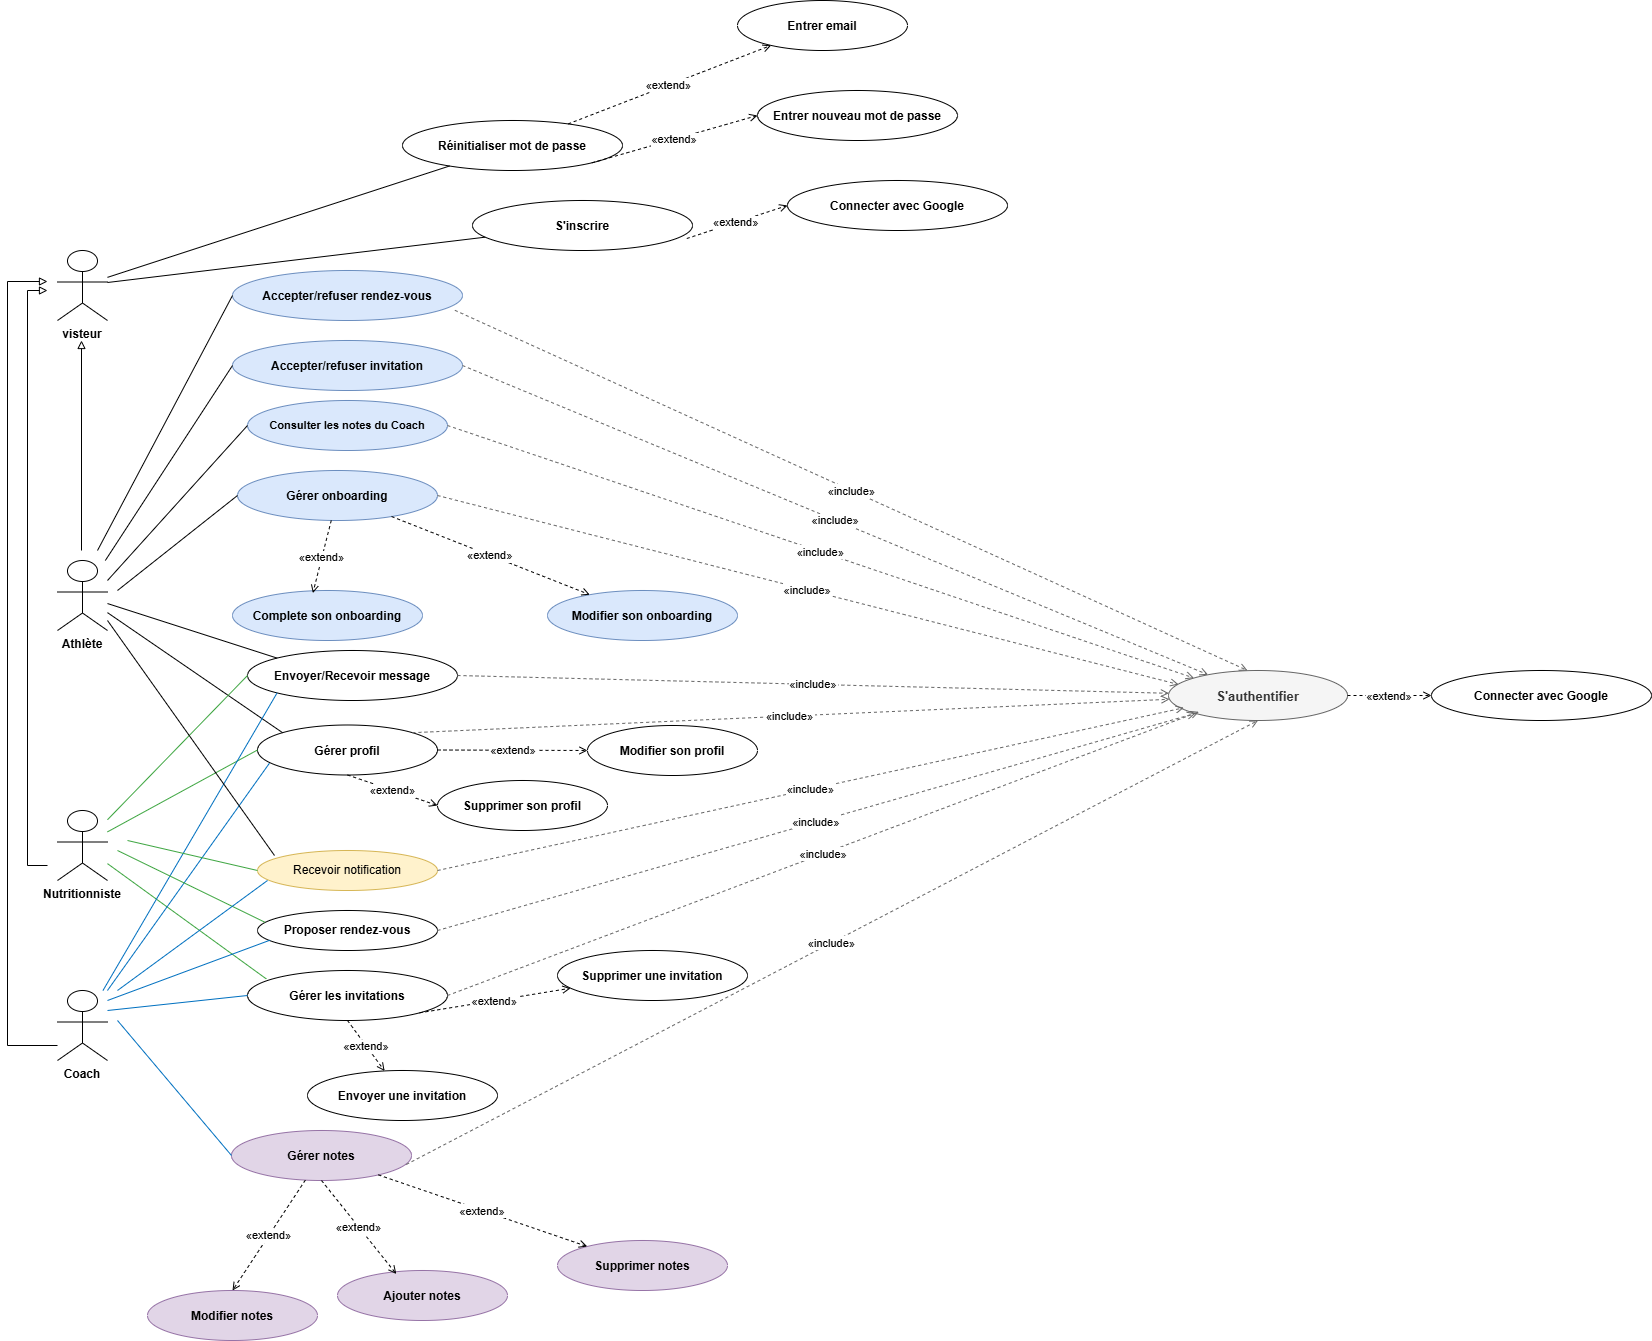
\includegraphics[width=0.9\textwidth]{images/usecasesprint1e.png}%
    }{%
        \fbox{\parbox[c][7cm][c]{0.9\textwidth}{\centering Ajouter l'image : \texttt{images/usecasesprint1e.png}}}%
    }
    \caption{Diagramme de cas d'utilisation du Sprint 1}
    \label{fig:cas_utilisation_sprint1}
\end{figure}

\FloatBarrier

\subsection{Description textuelle des cas d’utilisation étendus du Sprint,1}

Chaque cas d’utilisation est décrit sous forme de tableau normalisé précisant l’acteur, l’objectif, les pré-conditions, le scénario nominal et les scénarios alternatifs.

\subsubsection*{CU1 : S’authentifier}


\begin{table}[H]
\centering
\caption{Description du cas d'utilisation : s'authentifier}
\label{tab:cas_authentifier}
\small
\renewcommand{\arraystretch}{1.25}
\setlength{\tabcolsep}{5pt}
\begin{tabularx}{\textwidth}{|>{\RaggedRight\arraybackslash}p{3.4cm}|>{\RaggedRight\arraybackslash}X|}
\hline
\textbf{Cas d'utilisation} & S'authentifier \\
\hline
\textbf{Acteur} & Visiteur \\
\hline
\textbf{Préconditions} &
\begin{minipage}[t]{\linewidth}
\vspace{2pt}
\begin{itemize}[leftmargin=*, topsep=0pt, itemsep=1pt]
    \item Le visiteur dispose d'un compte enregistré dans le système.
    \item Le visiteur accède à la page de connexion de l'application UFitPal.
\end{itemize}
\vspace{2pt}
\end{minipage} \\
\hline
\textbf{Postcondition} &
\begin{minipage}[t]{\linewidth}
\vspace{2pt}
\begin{itemize}[leftmargin=*, topsep=0pt, itemsep=1pt]
    \item Le visiteur est authentifié et redirigé vers son tableau de bord selon son rôle (Athlète, Coach ou Nutritionniste).
   
\end{itemize}
\vspace{2pt}
\end{minipage} \\
\hline
\textbf{Scénario nominal} &
\begin{minipage}[t]{\linewidth}
\vspace{2pt}
\begin{enumerate}[label=\arabic*., leftmargin=*, topsep=0pt, itemsep=1pt]
    \item Le visiteur ouvre la page de connexion.
    \item Le système affiche le formulaire de connexion.
    \item Le visiteur saisit son adresse email et son mot de passe. 
    \item Le visiteur clique sur le bouton « Se connecter ».
    \item Le système vérifie les identifiants .
    \item Le système redirige le visiteur vers son tableau de bord.
\end{enumerate}
\vspace{2pt}
\end{minipage} \\
\hline
\textbf{Scénario alternatif} &
\begin{minipage}[t]{\linewidth}
\vspace{2pt}
\begin{itemize}[leftmargin=*, topsep=0pt, itemsep=1pt]
    \item \textbf{Connexion via Google OAuth} :
    \begin{itemize}[leftmargin=*, topsep=1pt, itemsep=1pt]
        \item Le visiteur clique sur « Connexion avec Google ».
        \item Le système redirige vers la page d'authentification Google.
        \item Après validation par Google, le système crée ou récupère le compte .
        \item Le visiteur est redirigé vers son tableau de bord.
    \end{itemize}
    \item  si l'email n'existe pas ou si le mot de passe est erroné, le système affiche « Email ou mot de passe incorrect » et la connexion échoue. Le visiteur peut réessayer.
\end{itemize}
\vspace{2pt}
\end{minipage} \\
\hline
\end{tabularx}
\end{table}

\subsubsection*{CU2 : S’inscrire}

% Figure removed: digrammeinscription.png image file not found
 
\begin{table}[H]
\sloppy
\centering
\caption{Description du cas d'utilisation : s'inscrire}
\label{tab:cas_inscrire}
\small
\renewcommand{\arraystretch}{1.25}
\setlength{\tabcolsep}{5pt}
\begin{tabularx}{\textwidth}{|>{\RaggedRight\arraybackslash}p{3.4cm}|>{\RaggedRight\arraybackslash}X|}
\hline
\textbf{Cas d'utilisation} & S'inscrire \\
\hline
\textbf{Acteur} & Visiteur \\
\hline
\textbf{Préconditions} &
\begin{minipage}[t]{\linewidth}
\vspace{2pt}
\begin{itemize}[leftmargin=*, topsep=0pt, itemsep=1pt]
    \item Le visiteur n'a pas encore de compte dans le système.
    \item Le visiteur accède à la page d'inscription de l'application UFitPal.
\end{itemize}
\vspace{2pt}
\end{minipage} \\
\hline
\textbf{Postcondition} &
\begin{minipage}[t]{\linewidth}
\vspace{2pt}
\begin{itemize}[leftmargin=*, topsep=0pt, itemsep=1pt]
    \item Un nouveau compte est créé avec le rôle choisi.
    \item Athlète : le visiteur est redirigé vers la page d'onboarding pour compléter son profil.
    \item Coach ou Nutritionniste : le visiteur est redirigé directement vers son tableau de bord.
\end{itemize}
\vspace{2pt}
\end{minipage} \\
\hline
\textbf{Scénario nominal} &
\begin{minipage}[t]{\linewidth}
\vspace{2pt}
\begin{enumerate}[label=\arabic*., leftmargin=*, topsep=0pt, itemsep=1pt]
    \item Le visiteur ouvre la page d'inscription.
    \item Le système affiche le formulaire d'inscription.
    \item Le visiteur choisit son rôle : Athlète, Coach ou Nutritionniste. 
    \item Le visiteur saisit ses informations personnelles : prénom, nom, email, mot de passe et confirmation. 
    \item Le visiteur clique sur « S'inscrire ».
    \item Le système crée le compte et connecte automatiquement le visiteur.
    \item Selon le rôle choisi :
    \begin{itemize}[leftmargin=*, topsep=1pt, itemsep=1pt]
        \item \textbf{Athlète} : le système redirige vers la page d'onboarding.
        \item \textbf{Coach ou Nutritionniste} : le système redirige vers le tableau de bord.
    \end{itemize}
\end{enumerate}
\vspace{2pt}
\end{minipage} \\
\hline
\textbf{Scénario alternatif} &
\begin{minipage}[t]{\linewidth}
\vspace{2pt}
\begin{itemize}[leftmargin=*, topsep=0pt, itemsep=1pt]
    \item \textbf{Inscription via Google OAuth} :
    \begin{itemize}[leftmargin=*, topsep=1pt, itemsep=1pt]
        \item Le visiteur choisit son rôle (Athlète / Coach / Nutritionniste), 
puis clique sur « Continuer avec Google ».
        \item Le système redirige vers la page d'authentification Google.
        \item Après validation, le système redirige selon le rôle : Coach vers \texttt{/coach}, Nutritionniste vers \texttt{/nutritionist}, Athlète vers \texttt{/athlete}.
    \end{itemize}
    \item  si  mot de passe et sa confirmation ne correspondent pas, le système affiche « Les mots de passe ne correspondent pas » et bloque la soumission.
    \item si le mot de passe contient moins de 8 caractères, le système affiche un message d'erreur.
    \item  si l'email est déjà utilisé, le système affiche un message d'erreur et invite le visiteur à se connecter.
\end{itemize}
\vspace{2pt}
\end{minipage} \\
\hline
\end{tabularx}
\fussy
\end{table}

\subsubsection*{CU3 : Réinitialiser le mot de passe}


\begin{table}[H]
\sloppy
\centering
\caption{Description du cas d'utilisation : réinitialiser le mot de passe}
\label{tab:cas_reinitialiser_mdp}
\small
\renewcommand{\arraystretch}{1.25}
\setlength{\tabcolsep}{5pt}
\begin{tabularx}{\textwidth}{|>{\RaggedRight\arraybackslash}p{3.4cm}|>{\RaggedRight\arraybackslash}X|}
\hline
\textbf{Cas d'utilisation} & Réinitialiser le mot de passe \\
\hline
\textbf{Acteur} & Visiteur \\
\hline
\textbf{Préconditions} &
\begin{minipage}[t]{\linewidth}
\vspace{2pt}
\begin{itemize}[leftmargin=*, topsep=0pt, itemsep=1pt]
    \item L'acteur possède un compte actif sur la plateforme.
    \item L'acteur a oublié son mot de passe et ne peut pas se connecter.
\end{itemize}
\vspace{2pt}
\end{minipage} \\
\hline
\textbf{Postcondition} &
Le mot de passe de l'utilisateur est modifié avec succès dans le système. L'utilisateur peut désormais se connecter avec son nouveau mot de passe. \\
\hline
\textbf{Scénario nominal} &
\begin{minipage}[t]{\linewidth}
\vspace{2pt}
\begin{enumerate}[leftmargin=*, topsep=0pt, itemsep=1pt]
    \item Le visiteur clique sur le lien « Mot de passe oublié ? » sur la page de connexion.
    \item Le système affiche un champ demandant l'adresse email.
    \item Le visiteur saisit son adresse email et valide.
    \item Le système vérifie que l'email existe, génère un code de vérification à 6 chiffres et l'envoie par email.
    \item Le système affiche un message de confirmation d'envoi indiquant que le code a été envoyé.
    \item Le visiteur ouvre l'email, récupère le code de 6 chiffres et le saisit dans le formulaire prévu à cet effet.
    \item Le système vérifie le code de vérification.
    \item Si le code est valide, le système affiche la page de définition du nouveau mot de passe.
    \item Le visiteur saisit son nouveau mot de passe, le confirme , puis clique sur \textit{Update password}.
    \item Le système met à jour le mot de passe et affiche un message de succès.
\end{enumerate}
\vspace{2pt}
\end{minipage} \\
\hline
\textbf{Scénario alternatif} &
\begin{minipage}[t]{\linewidth}
\vspace{2pt}
\begin{itemize}[leftmargin=*, topsep=0pt, itemsep=1pt]
    \item si l'email n'est pas reconnu, le système affiche un message d'erreur ou un message neutre indiquant qu'un lien a été envoyé.
    \item si le lien n'est plus valide, le système indique que le lien n'est plus valide et propose de recommencer la procédure.
    \item si le mot de passe est faible ou que les champs ne correspondent pas, le système affiche un message d'erreur et demande une nouvelle saisie.
\end{itemize}
\vspace{2pt}
\end{minipage} \\
\hline
\end{tabularx}
\fussy
\end{table}

\subsubsection*{CU4 : Gérer l’onboarding}


\begin{table}[H]
\centering
\caption{Description du cas d'utilisation : gérer onboarding}
\label{tab:cas_gerer_onboarding}
\small
\renewcommand{\arraystretch}{1.25}
\setlength{\tabcolsep}{5pt}
\begin{tabularx}{\textwidth}{|>{\RaggedRight\arraybackslash}p{3.4cm}|>{\RaggedRight\arraybackslash}X|}
\hline
\textbf{Cas d'utilisation} & Gérer onboarding \\
\hline
\textbf{Acteur} & Athlète \\
\hline
\textbf{Préconditions} &
\begin{minipage}[t]{\linewidth}
\vspace{2pt}
\begin{itemize}[leftmargin=*, topsep=0pt, itemsep=1pt]
    \item L'athlète a créé un compte et est actuellement connecté à l'application.
    \item L'athlète accède à l'espace lié à son profil personnel.
\end{itemize}
\vspace{2pt}
\end{minipage} \\
\hline
\textbf{Postcondition} &
\begin{minipage}[t]{\linewidth}
\vspace{2pt}
\begin{itemize}[leftmargin=*, topsep=0pt, itemsep=1pt]
    \item Les informations physiques, les objectifs sportifs et les données personnelles de l'athlète sont enregistrés et à jour dans le système.
\end{itemize}
\vspace{2pt}
\end{minipage} \\
\hline
\textbf{Scénario nominal} &
\begin{minipage}[t]{\linewidth}
\vspace{2pt}
\begin{enumerate}[label=\arabic*., leftmargin=*, topsep=0pt, itemsep=1pt]
    \item L'athlète accède à la rubrique dédiée à son profil ou y est redirigé automatiquement s'il s'agit de sa première connexion.
    \item Le système récupère les données existantes de l'athlète et vérifie si le profil a déjà été configuré par le passé.
    \item Selon l'état du profil, l'une des actions suivantes est déclenchée :
    \begin{itemize}[leftmargin=*, topsep=1pt, itemsep=1pt]
        \item \textbf{Première configuration} : le système affiche un questionnaire vide. L'athlète remplit ses informations obligatoires (âge, taille, poids, objectif principal, etc.). 
        \item \textbf{Mise à jour} : le système affiche le formulaire pré-rempli avec les anciennes données. L'athlète modifie uniquement les informations souhaitées. 
    \end{itemize}
    \item L'athlète clique sur le bouton de validation pour soumettre ses informations.
    \item Le système calcule automatiquement l'Indice de Masse Corporelle (IMC) en arrière-plan à partir du poids et de la taille fournis.
    \item Le système met à jour la base de données et marque officiellement le profil comme étant « complété ».
    \item Le système affiche un message de confirmation validant la réussite de l'enregistrement.
\end{enumerate}
\vspace{2pt}
\end{minipage} \\
\hline
\textbf{Scénario alternatif} &
\begin{minipage}[t]{\linewidth}
\vspace{2pt}
\begin{itemize}[leftmargin=*, topsep=0pt, itemsep=1pt]
    \item  si un champ obligatoire (comme le poids, la taille ou l'objectif) est laissé vide, le système ne valide pas les modifications et souligne les champs manquants en rouge.
    \item  si l'athlète quitte la page ou annule avant validation, le système annule l'opération et conserve les anciennes informations ou le statut non complété.
\end{itemize}
\vspace{2pt}
\end{minipage} \\
\hline
\end{tabularx}
\end{table}

\subsubsection*{CU5 : Gérer les invitations}

\begingroup
\setlength{\emergencystretch}{3em}


\begin{table}[H]
\sloppy
\centering
\caption{Description du cas d'utilisation : gérer les invitations}
\label{tab:cas_gerer_invitations}
\small
\renewcommand{\arraystretch}{1.25}
\setlength{\tabcolsep}{5pt}
\begin{tabularx}{\textwidth}{|>{\RaggedRight\arraybackslash}p{3.4cm}|>{\RaggedRight\arraybackslash}X|}
\hline
\textbf{Cas d'utilisation} & Gérer les invitations \\
\hline
\textbf{Acteur} & Coach, Nutritionniste \\
\hline
\textbf{Préconditions} &
\begin{minipage}[t]{\linewidth}\sloppy
\vspace{2pt}
\begin{itemize}[leftmargin=*, topsep=0pt, itemsep=1pt]
    \item Le professionnel (Coach ou Nutritionniste) est authentifié et connecté.
    \item Le professionnel accède à son interface de gestion des clients / athlètes.
\end{itemize}
\vspace{2pt}
\end{minipage} \\
\hline
\textbf{Postcondition} &
\begin{minipage}[t]{\linewidth}\sloppy
\vspace{2pt}
\begin{itemize}[leftmargin=*, topsep=0pt, itemsep=1pt]
    \item L'état des invitations est mis à jour dans le système : une nouvelle invitation est créée et mise en attente, ou une invitation existante est annulée/supprimée.
\end{itemize}
\vspace{2pt}
\end{minipage} \\
\hline
\textbf{Scénario nominal} &
\begin{minipage}[t]{\linewidth}\sloppy
\vspace{2pt}
\begin{enumerate}[label=\arabic*., leftmargin=*, topsep=0pt, itemsep=1pt]
    \item Le professionnel ouvre l'interface de gestion de ses clients.
    \item Le système affiche la liste des clients actuels ainsi que la liste des invitations en attente.
    \item Le professionnel sélectionne une action à effectuer :
    \begin{itemize}[leftmargin=*, topsep=1pt, itemsep=1pt]
        \item \textbf{Ajouter un nouvel athlète} : cliquer sur le bouton permettant d'inviter un client. 
        \item \textbf{Annuler une demande} : sélectionner une invitation en attente (ou un lien existant) et cliquer sur l'icône de suppression. 
    \end{itemize}
    \item Selon l'action choisie :
    \begin{itemize}[leftmargin=*, topsep=1pt, itemsep=1pt]
        \item \textbf{Envoyer} : le professionnel remplit le formulaire (ex. : adresse email de l'athlète), puis valide l'envoi.
        \item \textbf{Supprimer} : le professionnel confirme la suppression via une boîte de dialogue de sécurité.
    \end{itemize}
    \item Le système traite la demande et met à jour la base de données en conséquence.
    \item Le système affiche un message de confirmation (succès de l'envoi ou de la suppression) et rafraîchit la liste affichée.
\end{enumerate}
\vspace{2pt}
\end{minipage} \\
\hline
\textbf{Scénario alternatif} &
\begin{minipage}[t]{\linewidth}\sloppy
\vspace{2pt}
\begin{itemize}[leftmargin=*, topsep=0pt, itemsep=1pt]
    \item  si le professionnel tente d'envoyer une invitation à une adresse email invalide ou à un utilisateur qui n'existe pas, le système affiche un message d'erreur et l'invitation n'est pas créée.
    \item  si le professionnel annule la confirmation de suppression dans la boîte de dialogue, le système ignore l'action et la liste reste inchangée.
\end{itemize}
\vspace{2pt}
\end{minipage} \\
\hline
\end{tabularx}
\fussy

\end{table}
\endgroup

\begingroup
\setlength{\emergencystretch}{3em}
\subsubsection*{CU6 : répondre aux invitations de suivi}

\begin{table}[H]
\sloppy
\centering
\caption{Description du cas d'utilisation : répondre aux invitations de suivi}
\label{tab:cas_repondre_invitations_suivi}
\small
\renewcommand{\arraystretch}{1.25}
\setlength{\tabcolsep}{5pt}
\begin{tabularx}{\textwidth}{|>{\RaggedRight\arraybackslash}p{3.4cm}|>{\RaggedRight\arraybackslash}X|}
\hline
\textbf{Cas d'utilisation} & Répondre aux invitations de suivi \\
\hline
\textbf{Acteur} & Athlète \\
\hline
\textbf{Préconditions} &
\begin{minipage}[t]{\linewidth}\sloppy
\vspace{2pt}
\begin{itemize}[leftmargin=*, topsep=0pt, itemsep=1pt]
    \item L'athlète a créé un compte et est actuellement connecté à l'application.
    \item Un Coach ou un Nutritionniste a préalablement envoyé une invitation de suivi à l'athlète.
\end{itemize}
\vspace{2pt}
\end{minipage} \\
\hline
\textbf{Postcondition} &
\begin{minipage}[t]{\linewidth}\sloppy
\vspace{2pt}
\begin{itemize}[leftmargin=*, topsep=0pt, itemsep=1pt]
    \item Le statut de l'invitation est mis à jour dans le système : il passe à « acceptée » ou « refusée ».
    \item Une notification est automatiquement envoyée au Coach/Nutritionniste l'informant de la réponse de l'athlète.
\end{itemize}
\vspace{2pt}
\end{minipage} \\
\hline
\textbf{Scénario nominal} &
\begin{minipage}[t]{\linewidth}\sloppy
\vspace{2pt}
\begin{enumerate}[label=\arabic*., leftmargin=*, topsep=0pt, itemsep=1pt]
    \item L'athlète accède à son tableau de bord personnel.
    \item Le système récupère automatiquement la liste des invitations en attente adressées à l'athlète.
    \item Le système affiche la section « Invitations en attente » contenant, pour chaque invitation : le nom et le prénom de l'expéditeur, le type de suivi proposé (Coach ou Nutritionniste) ainsi que deux boutons d'action : Accepter et Refuser.
    \item L'athlète clique sur le bouton « Accepter » pour une invitation donnée.
    \item Le système vérifie que l'invitation existe, qu'elle appartient bien à l'athlète connecté et que son statut est toujours « en attente ».
    \item Le système enregistre l'acceptation et active le lien de suivi entre l'athlète et le Coach/Nutritionniste.
    \item Le système envoie une notification au Coach/Nutritionniste avec le message : « \{Nom de l'athlète\} a accepté votre invitation de suivi. »
    \item Le système actualise l'affichage et présente un message de confirmation validant la réussite de l'opération.
    \item L'invitation disparaît de la section « Invitations en attente » et le Coach/Nutritionniste apparaît désormais dans la carte « Mon Coach » ou « Mon Nutritionniste » du tableau de bord.
\end{enumerate}
\vspace{2pt}
\end{minipage} \\
\hline
\textbf{Scénario alternatif} &
\begin{minipage}[t]{\linewidth}\sloppy
\vspace{2pt}
\begin{itemize}[leftmargin=*, topsep=0pt, itemsep=1pt]
    \item  si l'athlète clique sur le bouton « Refuser », le système enregistre le refus et envoie une notification au Coach/Nutritionniste : « \{Nom de l'athlète\} a refusé votre invitation de suivi. » L'invitation disparaît de la liste.
    \item  si l'athlète tente de répondre à une invitation à laquelle il a déjà répondu, le système ne valide pas l'opération et affiche le message « Déjà répondu ».
    \item  si l'athlète n'a reçu aucune invitation, la section « Invitations en attente » ne s'affiche pas sur le tableau de bord.
\end{itemize}
\vspace{2pt}
\end{minipage} \\
\hline
\end{tabularx}
\fussy
\end{table}
\endgroup
\subsubsection*{CU7 : Gérer les notes de session}


\begin{table}[H]
\centering
\caption{Cas d'utilisation : Gérer les notes de session}
\label{tab:cas_gerer_notes_session}
\begin{tabular}{|p{4cm}|p{10cm}|}
\hline
\textbf{Cas d'utilisation} & Gérer les notes de session \\
\hline
\textbf{Acteur} & Coach \\
\hline
\textbf{Préconditions} &
\begin{minipage}[t]{\linewidth}
\vspace{2pt}
\begin{itemize}[leftmargin=*, topsep=0pt, itemsep=1pt]
    \item Le coach est authentifié et accède à son tableau de bord.
    \item Le coach dispose d'au moins un athlète dans sa liste de clients.
\end{itemize}
\vspace{2pt}
\end{minipage} \\
\hline
\textbf{Postcondition} & La note de session est enregistrée, modifiée ou supprimée et la liste est mise à jour en conséquence. \\
\hline
\textbf{Scénario nominal} &
\begin{minipage}[t]{\linewidth}
\vspace{2pt}
\begin{enumerate}[leftmargin=*, topsep=0pt, itemsep=1pt]
    \item Le coach accède à la section \textit{Session Notes} depuis le menu de navigation.
    \item Le système affiche la liste des notes existantes regroupées par athlète.
    \item Le coach ajoute, modifie ou supprime une note selon son besoin.
    \item Le système enregistre les modifications et met à jour la liste.
\end{enumerate}
\vspace{2pt}
\end{minipage} \\
\hline
\textbf{Scénario alternatif} &
\begin{minipage}[t]{\linewidth}
\vspace{2pt}
\begin{itemize}[leftmargin=*, topsep=0pt, itemsep=1pt]
    \item Si le coach annule la saisie, le système ferme le formulaire sans enregistrer.
    \item Si aucun client n'est sélectionné, le système empêche l'enregistrement de la note.
\end{itemize}
\vspace{2pt}
\end{minipage} \\
\hline
\end{tabular}
\end{table}

\begingroup
\setlength{\emergencystretch}{3em}
\subsubsection*{CU8 : Gérer la messagerie}

\begin{table}[H]
\sloppy
\centering
\caption{Description du cas d'utilisation : gérer la messagerie}
\label{tab:cas_gerer_messagerie}
\small
\renewcommand{\arraystretch}{1.25}
\setlength{\tabcolsep}{5pt}
\begin{tabularx}{\textwidth}{|>{\RaggedRight\arraybackslash}p{3.4cm}|>{\RaggedRight\arraybackslash}X|}
\hline
\textbf{Cas d'utilisation} & Gérer la messagerie \\
\hline
\textbf{Acteur} & Acteur connecté (Athlète, Coach ou Nutritionniste) \\
\hline
\textbf{Préconditions} &
\begin{minipage}[t]{\linewidth}\sloppy
\vspace{2pt}
\begin{itemize}[leftmargin=*, topsep=0pt, itemsep=1pt]
    \item L'utilisateur est connecté.
    \item Un lien de suivi est actif entre l'expéditeur et le destinataire.
\end{itemize}
\vspace{2pt}
\end{minipage} \\
\hline
\textbf{Postcondition} &
\begin{minipage}[t]{\linewidth}\sloppy
\vspace{2pt}
\begin{itemize}[leftmargin=*, topsep=0pt, itemsep=1pt]
    \item Le message est transmis et le destinataire reçoit une notification de nouveau message.
\end{itemize}
\vspace{2pt}
\end{minipage} \\
\hline
\textbf{Scénario nominal} &
\begin{minipage}[t]{\linewidth}\sloppy
\vspace{2pt}
\begin{enumerate}[label=\arabic*., leftmargin=*, topsep=0pt, itemsep=1pt]
    \item L'utilisateur accède à la messagerie et sélectionne son correspondant.
    \item Le système affiche l'historique de leur conversation.
    \item L'utilisateur saisit son message et clique sur Envoyer.
    \item Le système valide l'envoi, affiche le message et notifie le destinataire.
\end{enumerate}
\vspace{2pt}
\end{minipage} \\
\hline
\textbf{Scénario alternatif} &
\begin{minipage}[t]{\linewidth}\sloppy
\vspace{2pt}
\begin{itemize}[leftmargin=*, topsep=0pt, itemsep=1pt]
    \item si aucun lien de suivi n'existe entre les deux utilisateurs, l'envoi du message est bloqué.
    \item  les messages reçus passent automatiquement au statut « lu » lorsque l'utilisateur ouvre la conversation.
\end{itemize}
\vspace{2pt}
\end{minipage} \\
\hline
\end{tabularx}
\fussy
\end{table}
\endgroup


\begingroup
\setlength{\emergencystretch}{3em}
\subsubsection*{CU9 : proposer un rendez-vous}

\begin{table}[H]
\sloppy
\centering
\caption{Description du cas d'utilisation : proposer un rendez-vous}
\label{tab:cas_proposer_rendez_vous}
\small
\renewcommand{\arraystretch}{1.25}
\setlength{\tabcolsep}{5pt}
\begin{tabularx}{\textwidth}{|>{\RaggedRight\arraybackslash}p{3.4cm}|>{\RaggedRight\arraybackslash}X|}
\hline
\textbf{Cas d'utilisation} & Proposer un rendez-vous \\
\hline
\textbf{Acteur} & Coach ou Nutritionniste \\
\hline
\textbf{Préconditions} &
\begin{minipage}[t]{\linewidth}\sloppy
\vspace{2pt}
\begin{itemize}[leftmargin=*, topsep=0pt, itemsep=1pt]
    \item L'utilisateur est connecté.
    \item Un lien de suivi actif existe avec l'athlète sélectionné.
\end{itemize}
\vspace{2pt}
\end{minipage} \\
\hline
\textbf{Postcondition} &
\begin{minipage}[t]{\linewidth}\sloppy
\vspace{2pt}
\begin{itemize}[leftmargin=*, topsep=0pt, itemsep=1pt]
    \item La proposition de rendez-vous est créée avec le statut « planifié » et est visible par l'athlète.
\end{itemize}
\vspace{2pt}
\end{minipage} \\
\hline
\textbf{Scénario nominal} &
\begin{minipage}[t]{\linewidth}\sloppy
\vspace{2pt}
\begin{enumerate}[label=\arabic*., leftmargin=*, topsep=0pt, itemsep=1pt]
    \item Le professionnel accède à son calendrier ou son espace de suivi.
    \item Il clique sur l'option pour programmer un rendez-vous et sélectionne son athlète.
    \item Il renseigne les informations requises : titre, date, heure de début et de fin, notes.
    \item Il valide la saisie.
    \item Le système vérifie la validité des informations et la présence du lien de suivi.
    \item Le système enregistre le rendez-vous sous le statut « planifié » et confirme le succès de l'opération.
\end{enumerate}
\vspace{2pt}
\end{minipage} \\
\hline
\textbf{Scénario alternatif} &
\begin{minipage}[t]{\linewidth}\sloppy
\vspace{2pt}
\begin{itemize}[leftmargin=*, topsep=0pt, itemsep=1pt]
    \item  si la date ou l'heure est invalide, ou si un champ obligatoire est manquant, le système bloque la validation et signale les erreurs à corriger.
\end{itemize}
\vspace{2pt}
\end{minipage} \\
\hline
\end{tabularx}
\fussy
\end{table}
\endgroup

\begingroup
\setlength{\emergencystretch}{3em}
\subsubsection*{CU10 : Répondre à une proposition de rendez-vous}

\begin{table}[H]
\sloppy
\centering
\caption{Description du cas d'utilisation : répondre à une proposition de rendez-vous}
\label{tab:cas_repondre_rendez_vous}
\small
\renewcommand{\arraystretch}{1.25}
\setlength{\tabcolsep}{5pt}
\begin{tabularx}{\textwidth}{|>{\RaggedRight\arraybackslash}p{3.4cm}|>{\RaggedRight\arraybackslash}X|}
\hline
\textbf{Cas d'utilisation} & Répondre à une proposition de rendez-vous \\
\hline
\textbf{Acteur} & Athlète \\
\hline
\textbf{Préconditions} &
\begin{minipage}[t]{\linewidth}\sloppy
\vspace{2pt}
\begin{itemize}[leftmargin=*, topsep=0pt, itemsep=1pt]
    \item L'athlète est connecté.
    \item Un rendez-vous proposé par son Coach ou Nutritionniste est en attente avec le statut « planifié ».
\end{itemize}
\vspace{2pt}
\end{minipage} \\
\hline
\textbf{Postcondition} &
\begin{minipage}[t]{\linewidth}\sloppy
\vspace{2pt}
\begin{itemize}[leftmargin=*, topsep=0pt, itemsep=1pt]
    \item Le rendez-vous passe au statut « confirmé » en cas d'acceptation ou « annulé » en cas de refus.
\end{itemize}
\vspace{2pt}
\end{minipage} \\
\hline
\textbf{Scénario nominal} &
\begin{minipage}[t]{\linewidth}\sloppy
\vspace{2pt}
\begin{enumerate}[label=\arabic*., leftmargin=*, topsep=0pt, itemsep=1pt]
    \item L'athlète accède à son tableau de bord et repère l'invitation de rendez-vous.
    \item Il clique sur le bouton Accepter.
    \item Le système vérifie que le rendez-vous est toujours disponible et n'a pas été modifié.
    \item Le système change le statut du rendez-vous en « confirmé ».
    \item Le système actualise le calendrier et affiche un message de validation.
\end{enumerate}
\vspace{2pt}
\end{minipage} \\
\hline
\textbf{Scénario alternatif} &
\begin{minipage}[t]{\linewidth}\sloppy
\vspace{2pt}
\begin{itemize}[leftmargin=*, topsep=0pt, itemsep=1pt]
    \item  si l'athlète clique sur Refuser. Le système enregistre l'annulation, passe le statut du rendez-vous à « annulé » et le retire des rendez-vous en attente.
    \item  si le rendez-vous a déjà été complété ou annulé par le professionnel, le système empêche l'action et affiche un message d'erreur.
\end{itemize}
\vspace{2pt}
\end{minipage} \\
\hline
\end{tabularx}
\fussy
\end{table}
\endgroup
\begingroup
\setlength{\emergencystretch}{3em}
\subsubsection*{CU11 : consulter les notes de suivi}
\begingroup
\setlength{\emergencystretch}{3em}
\begin{table}[H]
\sloppy
\centering
\caption{Description du cas d'utilisation : consulter les notes de suivi}
\label{tab:cas_consulter_notes_suivi}
\small
\renewcommand{\arraystretch}{1.25}
\setlength{\tabcolsep}{5pt}
\begin{tabularx}{\textwidth}{|>{\RaggedRight\arraybackslash}p{3.4cm}|>{\RaggedRight\arraybackslash}X|}
\hline
\textbf{Cas d'utilisation} & Consulter les notes de suivi \\
\hline
\textbf{Acteur} & Athlète \\
\hline
\textbf{Préconditions} &
\begin{minipage}[t]{\linewidth}\sloppy
\vspace{2pt}
\begin{itemize}[leftmargin=*, topsep=0pt, itemsep=1pt]
    \item L'athlète est connecté.
    \item L'athlète possède un lien de suivi actif avec un Coach.
\end{itemize}
\vspace{2pt}
\end{minipage} \\
\hline
\textbf{Postcondition} &
\begin{minipage}[t]{\linewidth}\sloppy
\vspace{2pt}
\begin{itemize}[leftmargin=*, topsep=0pt, itemsep=1pt]
    \item Les remarques et consignes du Coach sont affichées à l'écran par ordre chronologique.
\end{itemize}
\vspace{2pt}
\end{minipage} \\
\hline
\textbf{Scénario nominal} &
\begin{minipage}[t]{\linewidth}\sloppy
\vspace{2pt}
\begin{enumerate}[label=\arabic*., leftmargin=*, topsep=0pt, itemsep=1pt]
    \item L'athlète accède à son tableau de bord principal.
    \item Le système récupère automatiquement l'ensemble des notes rédigées par son Coach.
    \item Le système trie ces notes de la plus récente à la plus ancienne.
    \item Le système affiche la liste des notes contenant la date, le nom du Coach et le contenu des observations.
    \item L'athlète consulte les informations.
\end{enumerate}
\vspace{2pt}
\end{minipage} \\
\hline
\textbf{Scénario alternatif} &
\begin{minipage}[t]{\linewidth}\sloppy
\vspace{2pt}
\begin{itemize}[leftmargin=*, topsep=0pt, itemsep=1pt]
    \item  si le Coach n'a rédigé aucune note, le système affiche un encadré vide avec la mention « Aucune note pour le moment ».
    \item  si aucun lien de suivi n'est établi avec un Coach, la section dédiée aux notes ne s'affiche pas sur l'écran de l'athlète.
\end{itemize}
\vspace{2pt}
\end{minipage} \\
\hline
\end{tabularx}
\fussy
\end{table}
\endgroup
\subsubsection*{CU12 : Recevoir des notifications en temps réel}

\begin{table}[H]
\centering
\caption{Cas d'utilisation : Recevoir des notifications en temps réel}
\label{tab:cas_recevoir_notifications_temps_reel}
\begin{tabular}{|p{4cm}|p{10cm}|}
\hline
\textbf{Cas d'utilisation} & Recevoir des notifications en temps réel \\
\hline
\textbf{Acteur} & Acteur connecté (Coach, Athlète, Nutritionniste) \\
\hline
\textbf{Préconditions} &
\begin{minipage}[t]{\linewidth}
\vspace{2pt}
\begin{itemize}[leftmargin=*, topsep=0pt, itemsep=1pt]
    \item L'acteur est authentifié et connecté à l'application.
\end{itemize}
\vspace{2pt}
\end{minipage} \\
\hline
\textbf{Postcondition} & L'acteur est informé en temps réel des événements qui le concernent et peut consulter l'ensemble de ses notifications. \\
\hline
\textbf{Scénario nominal} &
\begin{minipage}[t]{\linewidth}
\vspace{2pt}
\begin{enumerate}[leftmargin=*, topsep=0pt, itemsep=1pt]
    \item Un événement est déclenché dans le système (réponse à une invitation, nouveau message).
    \item Le système génère une notification et l'envoie en temps réel à l'acteur concerné.
    \item Le compteur de notifications s'incrémente dans la barre de navigation.
    \item L'acteur clique sur l'icône de notification.
    \item Le système affiche la liste des notifications avec leur contenu et leur date.
\end{enumerate}
\vspace{2pt}
\end{minipage} \\
\hline
\textbf{Scénario alternatif} &
\begin{minipage}[t]{\linewidth}
\vspace{2pt}
\begin{itemize}[leftmargin=*, topsep=0pt, itemsep=1pt]
    \item Si l'acteur n'est pas connecté au moment de l'événement, la notification est conservée et affichée lors de sa prochaine connexion.
    \item Si aucune notification n'est disponible, le système affiche un message indiquant qu'il n'y a aucune nouvelle notification.
\end{itemize}
\vspace{2pt}
\end{minipage} \\
\hline
\end{tabular}
\end{table}
\endgroup
\section{Conception}

Cette partie est consacrée à la modélisation et à la conception du système. Nous y exposons les diagrammes de séquence détaillant la dynamique des scénarios ainsi que le diagramme de classes global illustrant l'architecture des fonctionnalités clés développées au cours de ce sprint.

\subsection{Diagrammes de séquence}

Les diagrammes de séquence décrivent la dynamique du système en représentant les interactions temporelles entre ses composants. La collaboration entre les différents objets s'effectue via des échanges de messages ordonnés. Lorsque ces objets sont associés à des classes logicielles, chaque message correspond à l'appel d'une opération ou d'une méthode spécifique.


\subsubsection*{Diagramme de séquence de l'inscription}
La figure~\ref{fig:sequence_inscription} modélise le processus d'inscription. Le visiteur peut s'enregistrer via un formulaire classique, avec validation des mots de passe et vérification de l'unicité de l'e-mail, ou via Google OAuth. Après création sécurisée du compte en base de données, le système connecte automatiquement l'utilisateur et le redirige vers le tableau de bord correspondant à son rôle : Athlète, Coach ou Nutritionniste.

\begin{figure}[H]
    \centering
    \IfFileExists{images/pfekhouloud_digramme_de_sequence d'inscription1.png}{%
        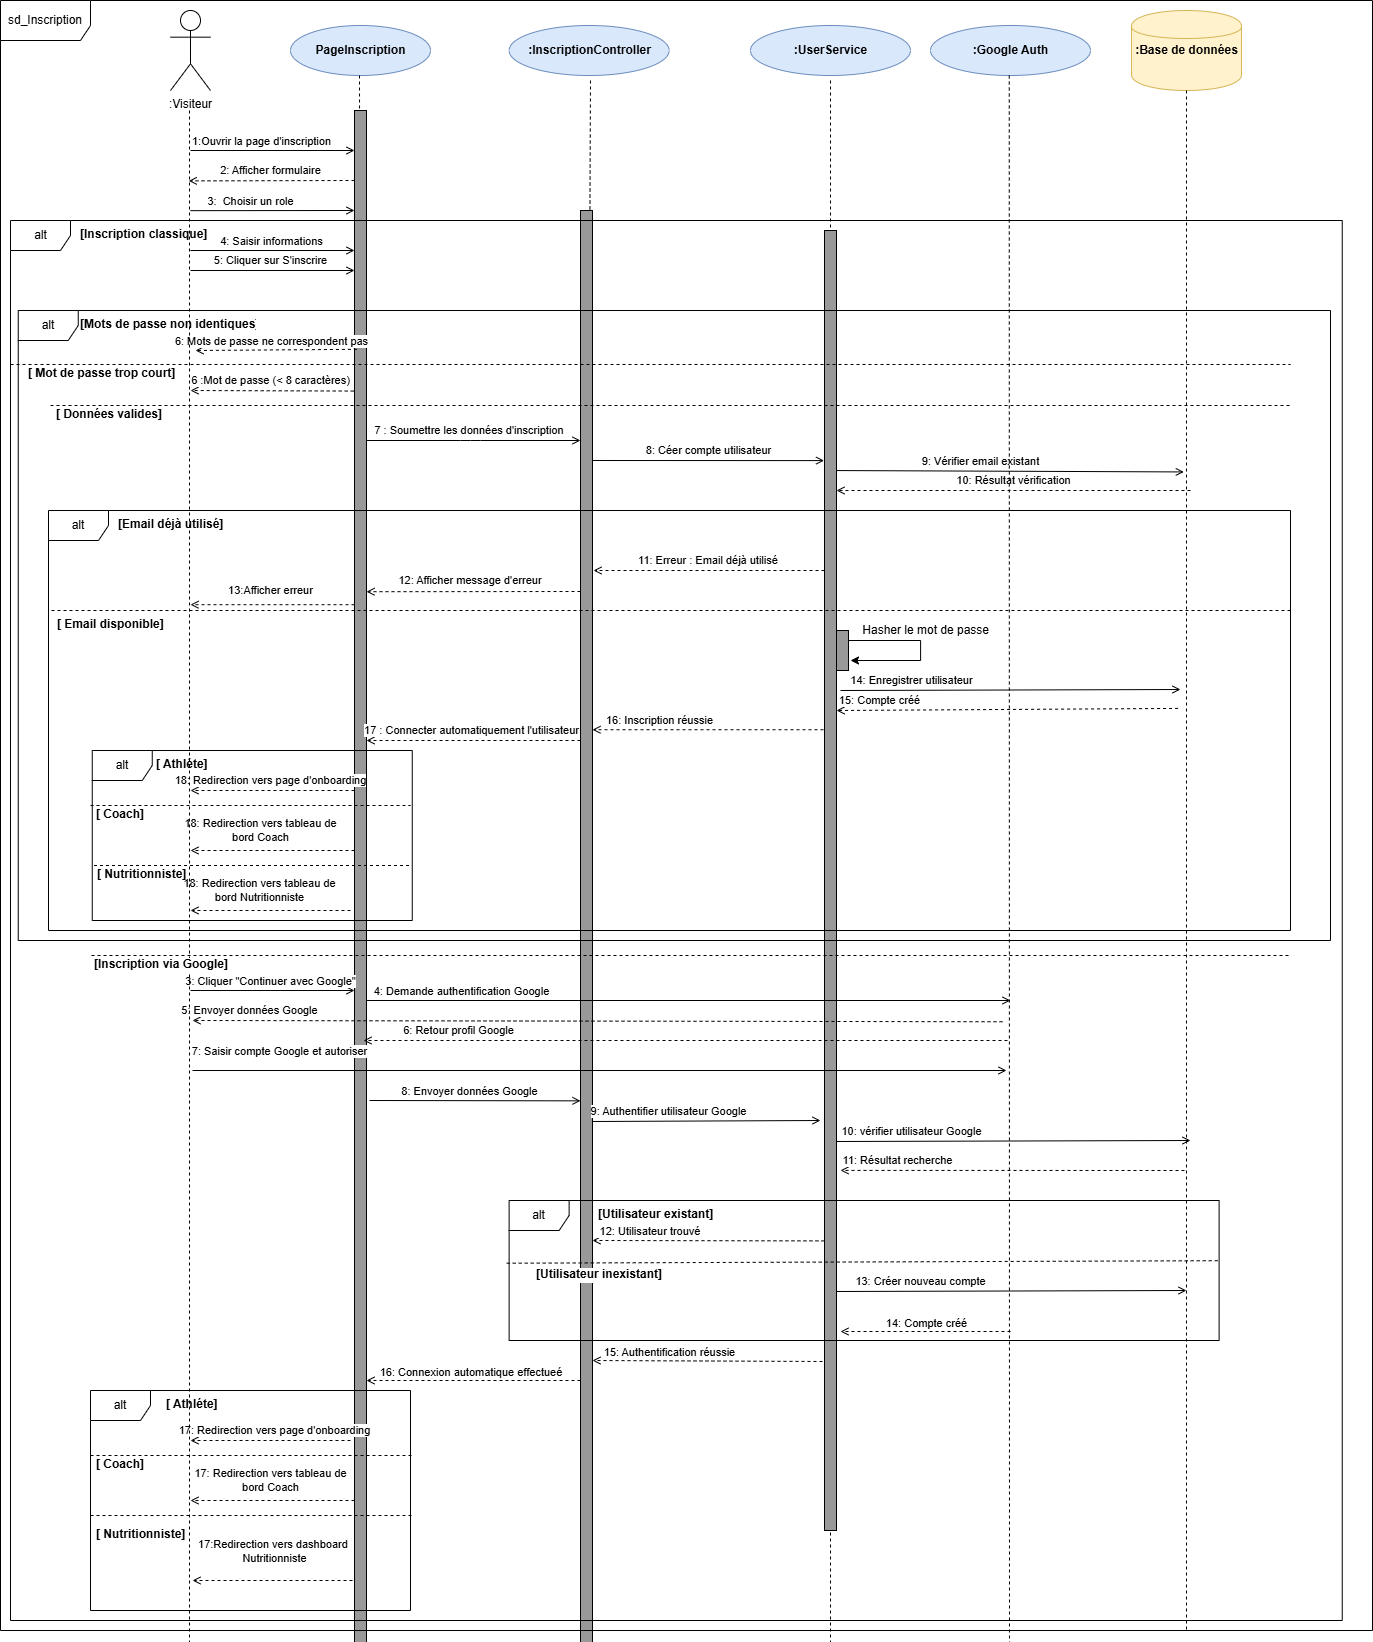
\includegraphics[width=0.9\textwidth]{images/pfekhouloud_digramme_de_sequence d'inscription1.png}%
    }{%
        \fbox{\parbox[c][6cm][c]{0.9\textwidth}{\centering Ajouter l'image : \texttt{images/diagramme\_sequence\_inscription.png}}}%
    }
    \caption{Diagramme de séquence de l'inscription}
    \label{fig:sequence_inscription}
\end{figure}

\subsubsection*{Diagramme de séquence de la connexion}
La figure~\ref{fig:sequence_connexion} présente le scénario d'authentification. L'utilisateur peut se connecter à l'aide de ses identifiants classiques ou via Google OAuth. Le système valide les informations de connexion auprès de la base de données : une authentification réussie redirige l'utilisateur vers son espace personnel, tandis qu'un échec d'authentification génère un message d'erreur.

\begin{figure}[H]
    \centering
    \IfFileExists{images/digramme_de_sequance_login.png}{%
        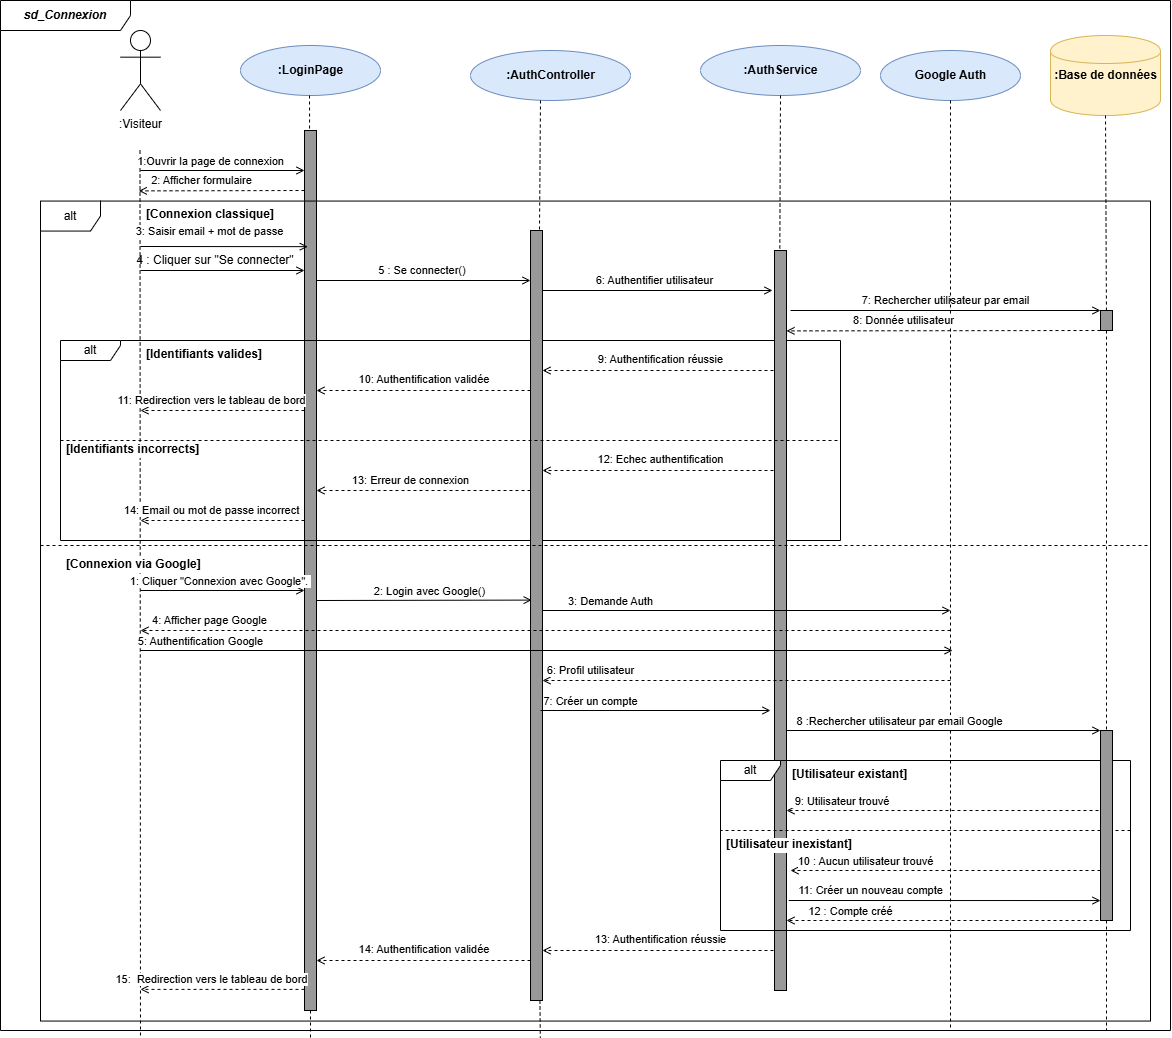
\includegraphics[width=0.9\textwidth]{images/digramme_de_sequance_login.png}%
    }{%
        \fbox{\parbox[c][6cm][c]{0.9\textwidth}{\centering Ajouter l'image : \texttt{images/diagramme\_sequence\_connexion.png}}}%
    }
    \caption{Diagramme de séquence de la connexion}
    \label{fig:sequence_connexion}
\end{figure}

\subsubsection*{Diagramme de séquence de la configuration de l'onboarding}
La figure~\ref{fig:sequence_onboarding} décrit la configuration de l'onboarding de l'athlète. Le système charge les données existantes de l'utilisateur pour pré-remplir le formulaire. Après validation des données physiques saisies, le système calcule l'Indice de Masse Corporelle (IMC) en arrière-plan, met à jour le profil dans la base de données et valide l'onboarding. L'annulation reste possible à tout moment pour préserver les anciennes données.

\begin{figure}[H]
    \centering
    \IfFileExists{images/digramme_de_sequance_modifier_onborading.png}{%
        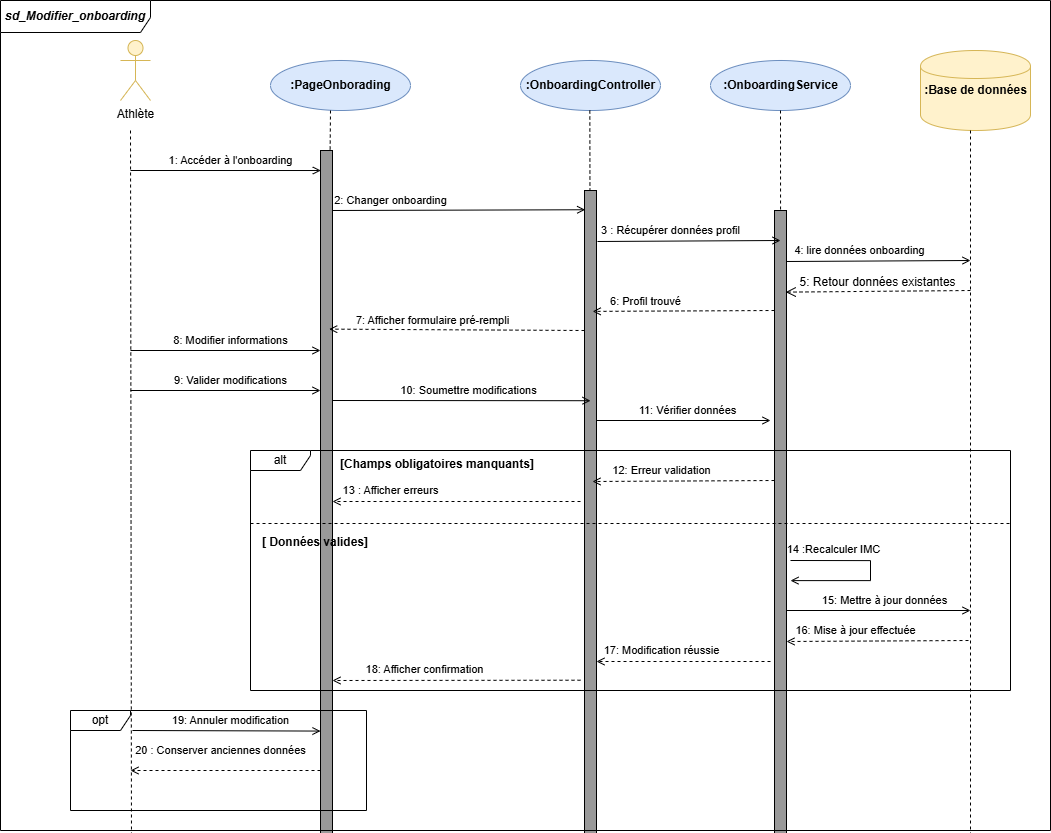
\includegraphics[width=0.9\textwidth]{images/digramme_de_sequance_modifier_onborading.png}%
    }{%
        \fbox{\parbox[c][6cm][c]{0.9\textwidth}{\centering Ajouter l'image : \texttt{images/diagramme\_sequence\_onboarding.png}}}%
    }
    \caption{Diagramme de séquence de la configuration de l'onboarding}
    \label{fig:sequence_onboarding}
\end{figure}

\subsubsection*{Diagramme de séquence de l'invitation d'un client}
La figure~\ref{fig:sequence_invitation_client} illustre le flux d'invitation d'un athlète par un professionnel, Coach ou Nutritionniste. Le système identifie l'athlète cible par son adresse e-mail, vérifie qu'aucune invitation active ou en attente n'est déjà en cours, puis enregistre l'invitation avec le statut « invité » avant de rafraîchir l'interface utilisateur.

\begin{figure}[H]
    \centering
    \IfFileExists{images/pfekhouloud digramme de classe-envoyer invitition2.png}{%
        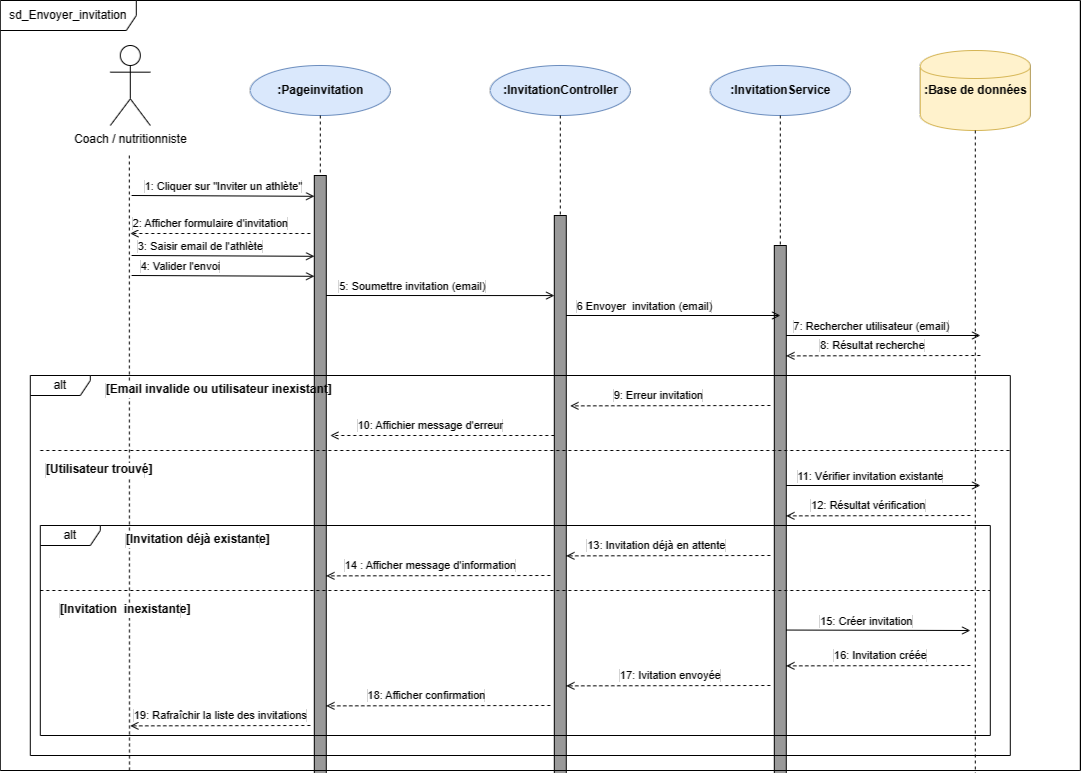
\includegraphics[width=0.9\textwidth]{images/pfekhouloud digramme de classe-envoyer invitition2.png}%
    }{%
        \fbox{\parbox[c][6cm][c]{0.9\textwidth}{\centering Ajouter l'image : \texttt{images/diagramme\_sequence\_invitation\_client.png}}}%
    }
    \caption{Diagramme de séquence de l'invitation d'un client}
    \label{fig:sequence_invitation_client}
\end{figure}

\subsection{Diagramme de classes du Sprint 1}
Le diagramme de classes présenté sur la figure~\ref{fig:diagramme_classes_sprint1} montre la structure statique des données développées durant ce premier sprint.

Elle repose sur la classe centrale \texttt{User}, dont les droits et accès sont définis par l'énumération \texttt{UserRole}. Pour l'Athlète, le profil est complété par ses \texttt{Mesures\_physiques} (poids, taille, IMC) ainsi que ses \texttt{Objectifs\_utilisateur} (niveau de fitness, blessures).
La classe \texttt{Suivi\_client} modélise la relation d'accompagnement : elle associe un athlète à son professionnel et sert de support à l'enregistrement des \texttt{Note\_session} et à la planification des \texttt{Rendez\_vous}. Enfin, la classe \texttt{Message} permet d'assurer les communications bidirectionnelles sécurisées entre les différents acteurs de la plateforme.
\begin{figure}[H]
    \centering
    \IfFileExists{images/de_classe-digramme-de-classe de sprint1.png}{%
        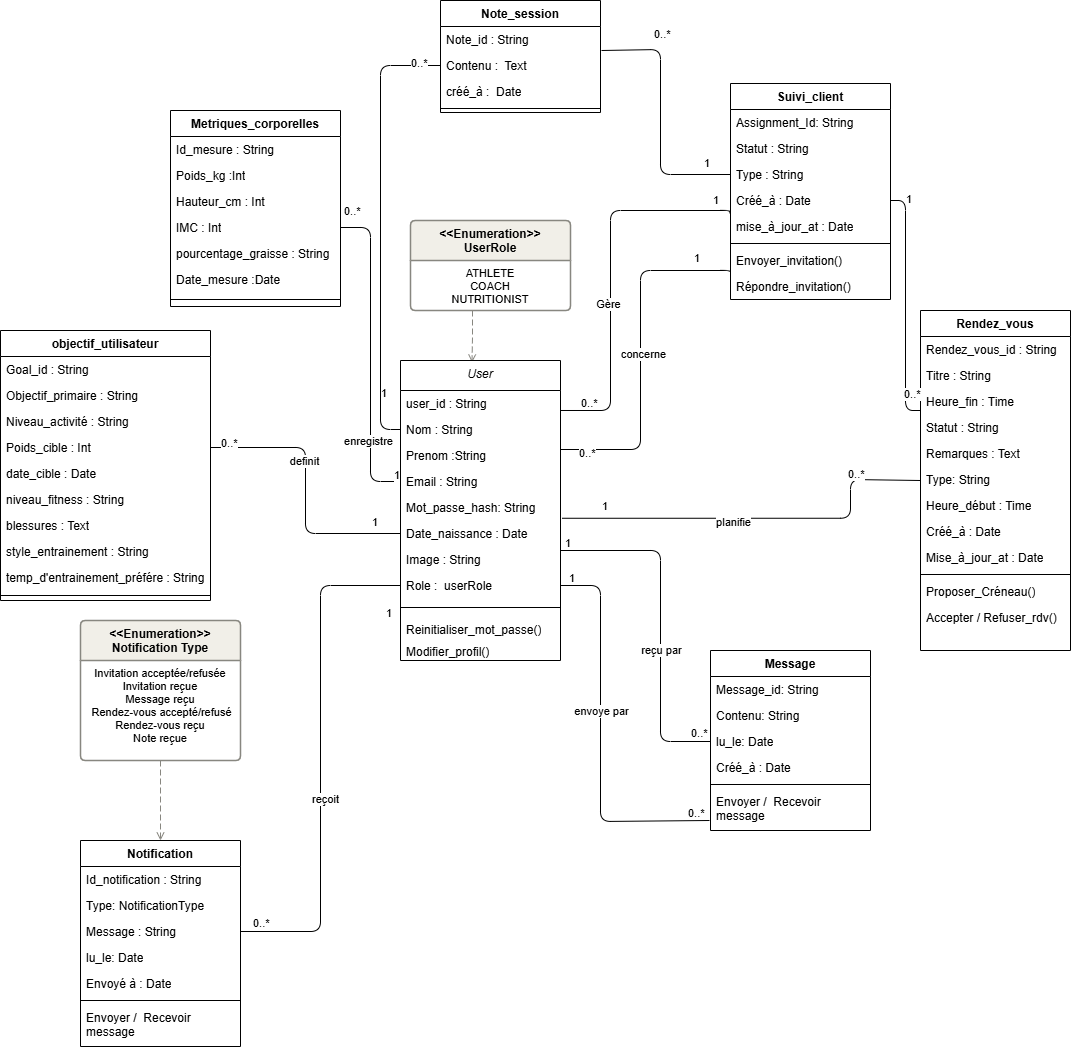
\includegraphics[width=0.95\textwidth]{images/de_classe-digramme-de-classe de sprint1.png}%
    }{%
        \fbox{\parbox[c][7cm][c]{0.95\textwidth}{\centering Ajouter l'image : \texttt{images/diagramme\_classes\_sprint1.png}}}%
    }
    \caption{Diagramme de classes du Sprint 1}
    \label{fig:diagramme_classes_sprint1}
\end{figure}

\section{Réalisation}

\subsection{Authentification (Sign in)}
L'utilisateur saisit son email et son mot de passe puis, en appuyant sur le bouton « Se connecter », il est redirigé vers l'espace personnel correspondant à son rôle. La figure~\ref{fig:interface_connexion} présente l'interface de connexion :

\begin{figure}[H]
    \centering
    \IfFileExists{images/sigin.png}{%
        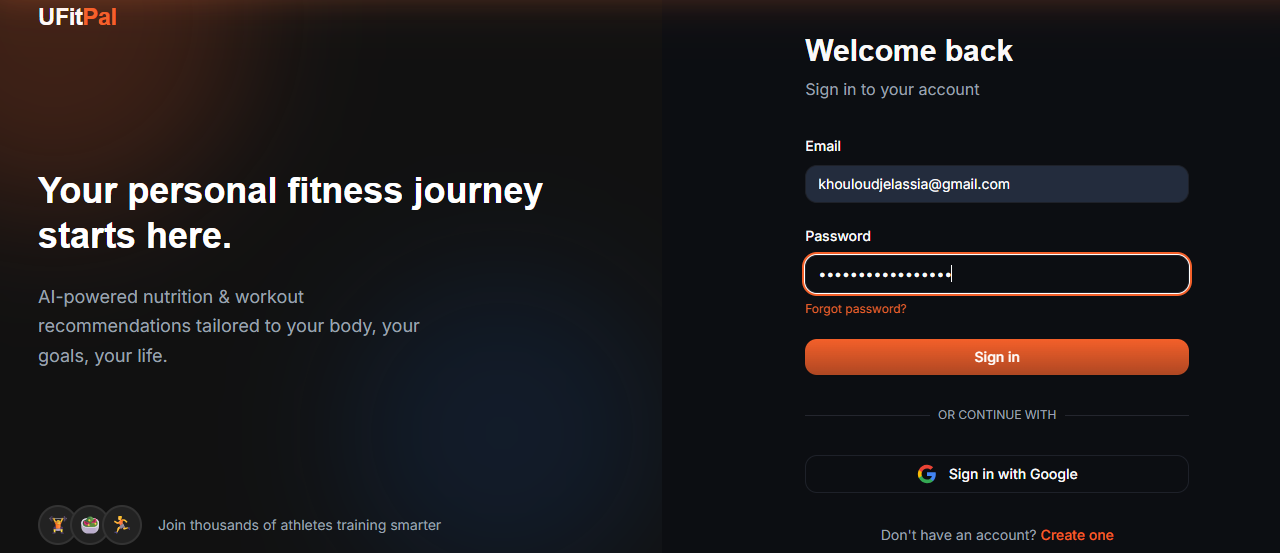
\includegraphics[width=0.85\textwidth]{images/sigin.png}%
    }{%
        \fbox{\parbox[c][6cm][c]{0.85\textwidth}{\centering Ajouter l'image : \texttt{images/interface\_connexion.png}}}%
    }
    \caption{Interface de connexion}
    \label{fig:interface_connexion}
\end{figure}

\subsection{Inscription (Sign up)}
L'utilisateur remplit le formulaire d'inscription en saisissant ses informations personnelles, son adresse email, son mot de passe et en choisissant son rôle au sein de la plateforme. Après validation via le bouton \textit{Create account}, le système crée le compte et redirige l'utilisateur vers l'espace adapté à son profil. La figure~\ref{fig:interface_inscription} présente l'interface d'inscription :
\begin{figure}[H]
    \centering
    \IfFileExists{images/sigup.png}{%
        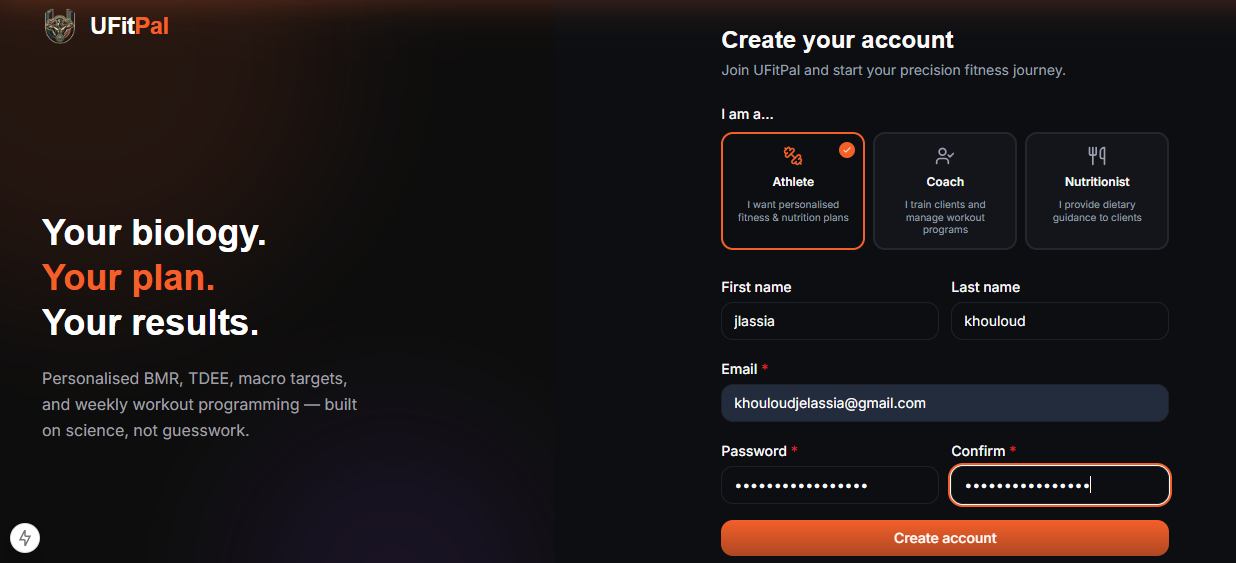
\includegraphics[width=0.85\textwidth]{images/sigup.png}%
    }{%
        \fbox{\parbox[c][6cm][c]{0.85\textwidth}{\centering Ajouter l'image : \texttt{images/interface\_inscription.png}}}%
    }
    \caption{Interface d'inscription}
    \label{fig:interface_inscription}
\end{figure}

\subsection{Réinitialisation du mot de passe}
La fonctionnalité de réinitialisation du mot de passe se déroule en plusieurs étapes. L'utilisateur saisit son adresse email afin de recevoir un code de vérification à 6 chiffres. Une fois le code reçu par email, il l'introduit dans le formulaire et définit un nouveau mot de passe avec confirmation. Après validation via le bouton \textit{Update password}, le mot de passe est mis à jour avec succès. Les figures~\ref{fig:forgot_password1}, \ref{fig:forgot_password2} et~\ref{fig:forgot_password3} illustrent respectivement la saisie de l'email, la réception du code et la mise à jour du mot de passe :

\begin{figure}[H]
    \centering
    \IfFileExists{images/forgetpassword1.png}{%
        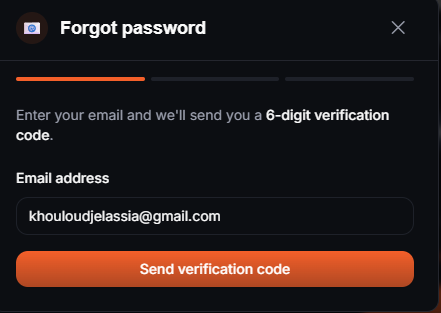
\includegraphics[width=0.85\textwidth]{images/forgetpassword1.png}%
    }{%
        \fbox{\parbox[c][6cm][c]{0.85\textwidth}{\centering Ajouter l'image : \texttt{images/forget\_password1.png}}}%
    }
    \caption{Saisie de l'adresse email}
    \label{fig:forgot_password1}
\end{figure}

\begin{figure}[H]
    \centering
    \IfFileExists{images/forgetpassword2.png}{%
        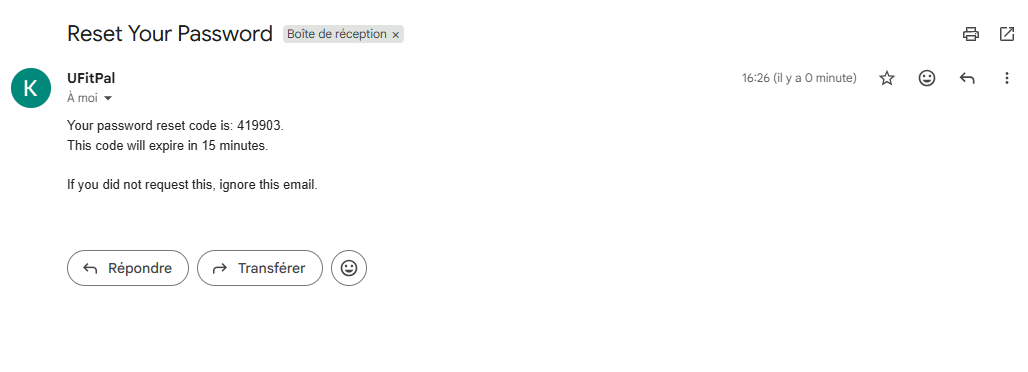
\includegraphics[width=0.85\textwidth]{images/forgetpassword2.png}%
    }{%
        \fbox{\parbox[c][6cm][c]{0.85\textwidth}{\centering Ajouter l'image : \texttt{images/forget\_password2.png}}}%
    }
    \caption{Saisie du code de vérification}
    \label{fig:forgot_password2}
\end{figure}

\begin{figure}[H]
    \centering
    \IfFileExists{images/forgetpassword3.png}{%
        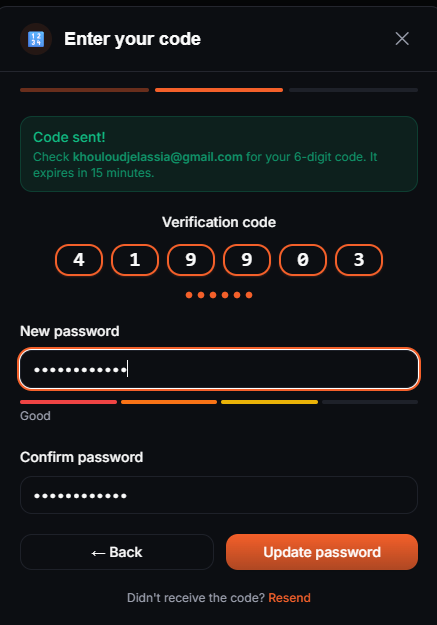
\includegraphics[width=0.85\textwidth]{images/forgetpassword3.png}%
    }{%
        \fbox{\parbox[c][6cm][c]{0.85\textwidth}{\centering Ajouter l'image : \texttt{images/forget\_password3.png}}}%
    }
    \caption{Mise à jour du mot de passe}
    \label{fig:forgot_password3}
\end{figure}
\subsection{Gestion des invitations}
Le coach peut inviter un client en recherchant son adresse email via la boîte de dialogue \textit{Invite Client}, puis en lui envoyant une invitation. Une fois l'invitation envoyée, le client apparaît dans la liste \textit{My Clients} avec un statut \textit{Pending} dans l'attente de sa réponse. Le coach reçoit ensuite une notification en temps réel l'informant de l'acceptation ou du refus de l'invitation. Les figures~\ref{fig:invite_client}, \ref{fig:liste_clients} et~\ref{fig:notifications} illustrent respectivement l'envoi de l'invitation, la liste des clients et les notifications reçues :

\begin{figure}[H]
    \centering
    \IfFileExists{images/inviteclient.png}{%
        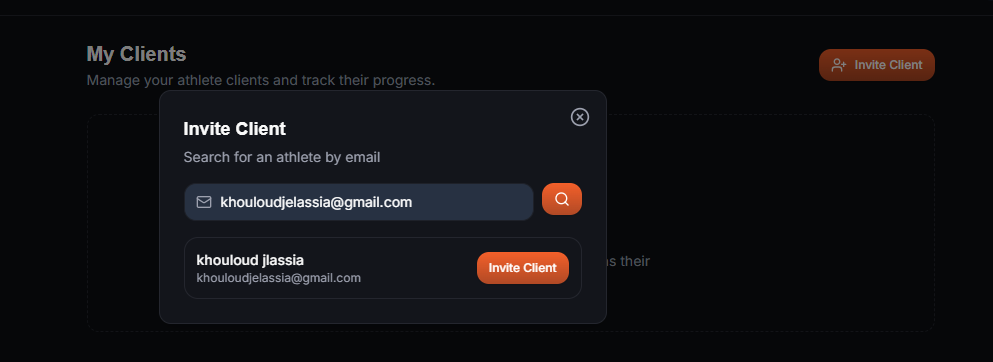
\includegraphics[width=0.85\textwidth]{images/inviteclient.png}%
    }{%
        \fbox{\parbox[c][6cm][c]{0.85\textwidth}{\centering Ajouter l'image : \texttt{images/invite\_client.png}}}%
    }
    \caption{Envoi d'une invitation à un client}
    \label{fig:invite_client}
\end{figure}

\begin{figure}[H]
    \centering
    \IfFileExists{images/consulterlistedeclient.png}{%
        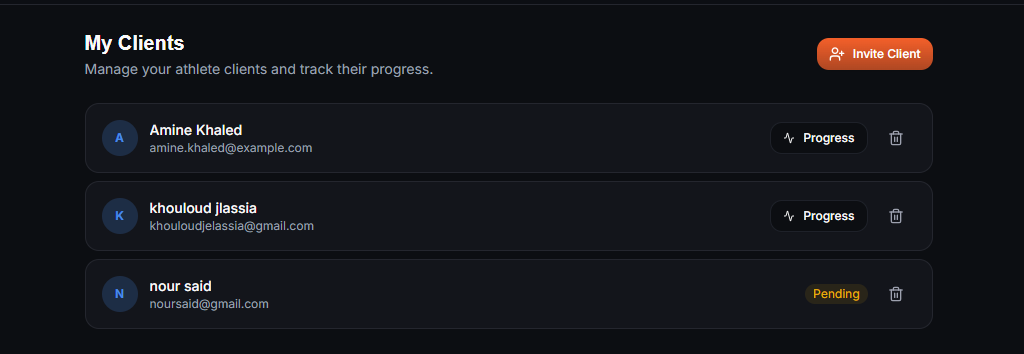
\includegraphics[width=0.85\textwidth]{images/consulterlistedeclient.png}%
    }{%
        \fbox{\parbox[c][6cm][c]{0.85\textwidth}{\centering Ajouter l'image : \texttt{images/consulterliste\_de\_client.png}}}%
    }
    \caption{Liste des clients du coach}
    \label{fig:liste_clients}
\end{figure}

\begin{figure}[H]
    \centering
    \IfFileExists{images/notification.png}{%
        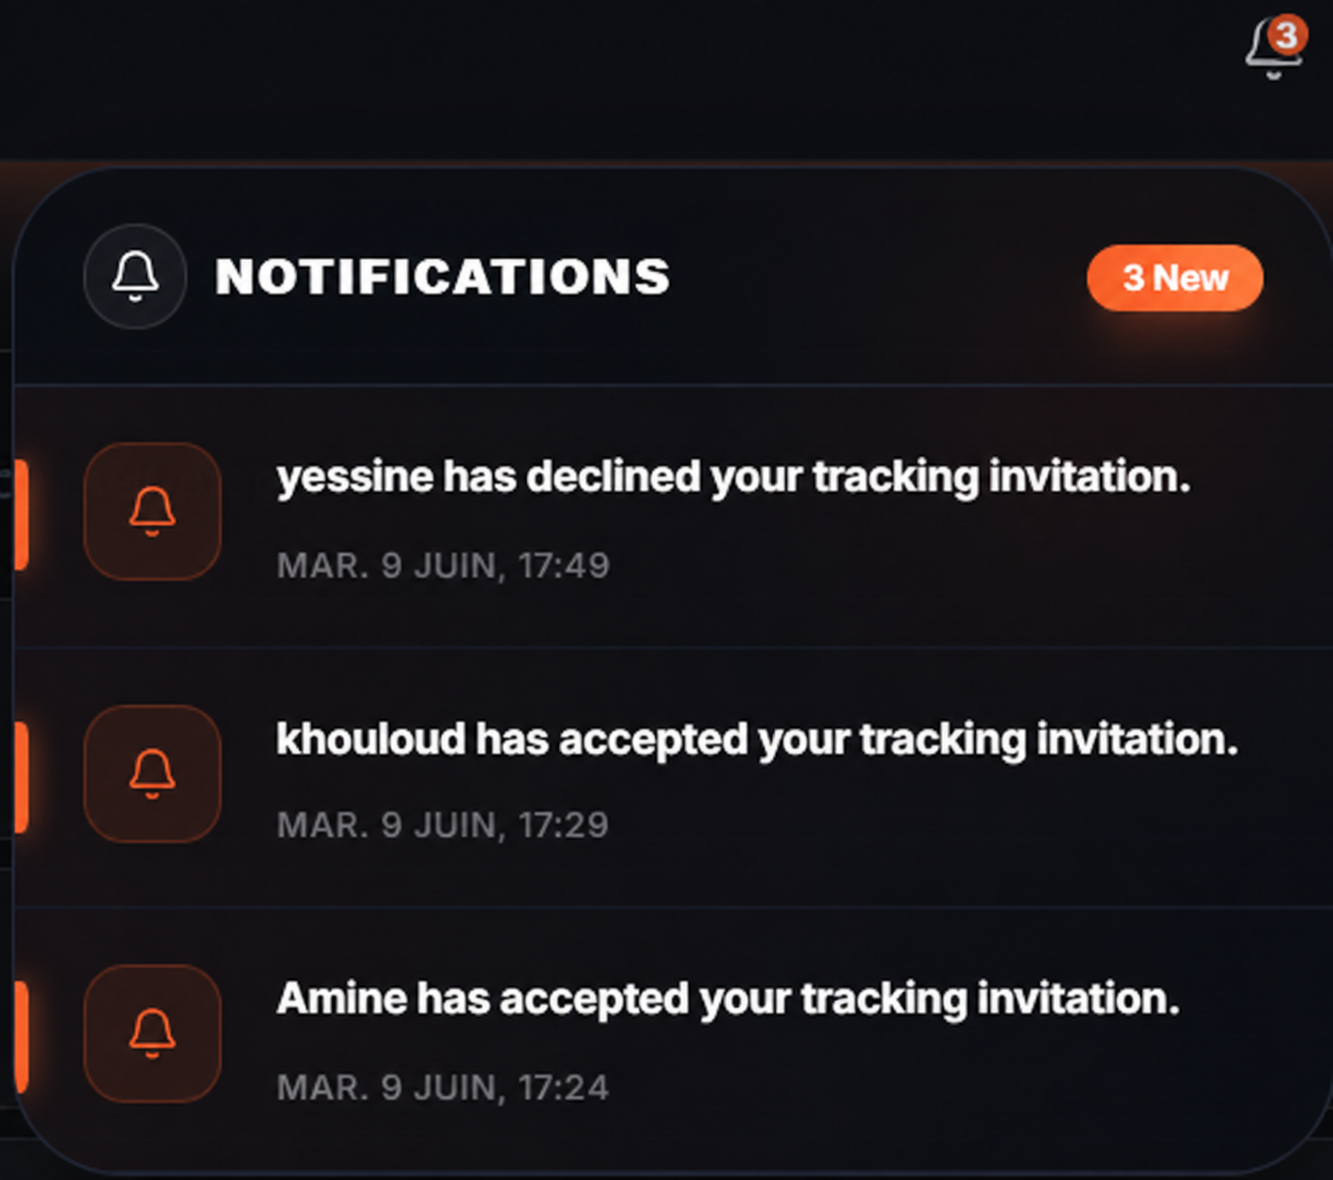
\includegraphics[width=0.85\textwidth]{images/notification.png}%
    }{%
        \fbox{\parbox[c][6cm][c]{0.85\textwidth}{\centering Ajouter l'image : \texttt{images/notification.png}}}%
    }
    \caption{Notifications reçues par le coach}
    \label{fig:notifications}
\end{figure}

\section{Conclusion}
Au cours de ce sprint, nous avons pu concevoir et développer les fonctionnalités principales du premier sprint de l'application UFitPal,
 à savoir l'inscription, la connexion, la réinitialisation du mot de passe, la gestion du profil, la gestion des invitations
  ainsi que la communication entre les différents acteurs de la plateforme. Le prochain chapitre traitera de la mise en œuvre du deuxième sprint, axé sur le suivi sportif et nutritionnel de l'athlète, la gestion des plans repas par le nutritionniste, 
et l'intégration de fonctionnalités d'intelligence artificielle et d'un chatbot IA pour des recommandations personnalisées.

\chapter*{Chapitre 4 : Release 2 : Sprint 2 — Suivi sportif, nutrition et intelligence artificielle}
\addcontentsline{toc}{chapter}{Chapitre 4 : Release 2 : Sprint 2 — Suivi sportif, nutrition et intelligence artificielle}

\setcounter{section}{0}

\FloatBarrier
\section{Introduction}
\vspace{-1em}
Ce chapitre est consacré au deuxième sprint de développement de l'application UFitPal. Il porte principalement sur les fonctionnalités liées au suivi sportif et nutritionnel de l'athlète, à la gestion des plans repas par le nutritionniste, ainsi qu'à l'intégration des premiers modules d'intelligence artificielle permettant d'améliorer la personnalisation de l'expérience utilisateur.

Ce chapitre suit la même organisation que le chapitre précédent. Nous présentons d'abord le backlog du Sprint 2, puis les spécifications fonctionnelles à travers les diagrammes et descriptions textuelles des cas d'utilisation. Ensuite, nous abordons la conception à l'aide des diagrammes de séquence et du diagramme de classes, avant de terminer par la réalisation des fonctionnalités développées.

\section{Sprint 2 backlog}

Le tableau suivant présente les \textit{user stories} retenues pour le Sprint~2, regroupées par thème fonctionnel et accompagnées de leur priorité.

{\small
\begin{longtable}{|
  >{\RaggedRight\arraybackslash}p{1.4cm}|
  >{\RaggedRight\arraybackslash}p{2.8cm}|
  >{\centering\arraybackslash}p{1.2cm}|
  >{\RaggedRight\arraybackslash}p{7.1cm}|
  >{\RaggedRight\arraybackslash}p{1.5cm}|
}

\hline
\textbf{Sprint} & \textbf{Thème} & \textbf{ID} & \textbf{User Story} & \textbf{Priorité} \\
\hline
\endfirsthead

\hline
\textbf{Sprint} & \textbf{Thème} & \textbf{ID} & \textbf{User Story} & \textbf{Priorité} \\
\hline
\endhead

\hline
\endfoot

\hline
\endlastfoot

Sprint 2 & Suivi Athlète & US 2.1 &
En tant qu'Athlète, je veux saisir mes séances sportives afin d'alimenter mon suivi. &
Élevée \\
\cline{2-5}

 & Suivi Athlète & US 2.2 &
En tant qu'Athlète, je veux enregistrer mon poids et mes performances afin de suivre mon évolution. &
Élevée \\
\cline{2-5}

 & Suivi Athlète & US 2.3 &
En tant qu'Athlète, je veux tenir mon journal alimentaire quotidien afin de suivre mes apports nutritionnels. &
Élevée \\
\cline{2-5}

 & Nutrition & US 2.4 &
En tant que Nutritionniste, je veux créer un plan repas et l'assigner à mon Athlète client afin de l'accompagner dans sa nutrition. &
Élevée \\
\cline{2-5}

 & Nutrition & US 2.5 &
En tant qu'Athlète, je veux consulter le plan repas créé par mon Nutritionniste afin de suivre ses recommandations. &
Élevée \\
\cline{2-5}

 & IA \& ML & US 2.6 &
En tant qu'Athlète, je veux voir mon score de risque d'abandon (churn) afin de prendre des mesures préventives. &
Moyenne \\
\cline{2-5}

 & IA \& ML & US 2.7 &
En tant qu'Athlète, je veux voir la prédiction d'évolution de mon poids afin de suivre ma trajectoire. &
Moyenne \\
\cline{2-5}

 & IA \& ML & US 2.8 &
En tant qu'Athlète, je veux voir la probabilité d'atteindre mon objectif fitness basée sur mon profil. &
Moyenne \\
\cline{2-5}

 & IA \& ML & US 2.9 &
En tant qu'Athlète, je veux détecter un plateau sportif afin d'adapter mon programme d'entraînement. &
Moyenne \\
\cline{2-5}

 & IA \& ML & US 2.10 &
En tant qu'Athlète, je veux consulter des recommandations issues d'un système rules-based fondé sur des formules scientifiques (Mifflin-St Jeor, ratios macronutriments, seuils IMC OMS). &
Moyenne \\
\cline{2-5}

 & IA \& ML & US 2.11 &
En tant qu'Athlète, je veux poser des questions à un chatbot IA afin d'obtenir des conseils personnalisés sur ma nutrition et mon entraînement. &
Moyenne \\
\hline

\end{longtable}
}

\section{Spécifications fonctionnelles}

\subsection{Diagramme de cas d'utilisation du Sprint 2}

\begin{figure}[H]
    \centering
    \IfFileExists{images/diagramme_cas_utilisation_sprint2.png}{%
        \includegraphics[width=0.9\textwidth]{images/diagramme_cas_utilisation_sprint2.png}%
    }{%
        \fbox{\parbox[c][7cm][c]{0.9\textwidth}{\centering Ajouter l'image : \texttt{images/diagramme\_cas\_utilisation\_sprint2.png}}}%
    }
    \caption{Diagramme de cas d'utilisation du Sprint 2}
    \label{fig:cas_utilisation_sprint2}
\end{figure}

\subsection{Description textuelle des cas d'utilisation du Sprint 2}

Cette partie présente les descriptions détaillées des cas d'utilisation du Sprint 2, notamment la gestion des activités sportives, le suivi de la progression, le journal alimentaire, les plans repas, les recommandations intelligentes et l'interaction avec le chatbot IA.

\begin{table}[H]
\sloppy
\centering
\caption{Description du cas d'utilisation : enregistrer son activité}
\label{tab:cas_enregistrer_activite}
\small
\renewcommand{\arraystretch}{1.25}
\setlength{\tabcolsep}{5pt}
\begin{tabularx}{\textwidth}{|>{\RaggedRight\arraybackslash}p{3.4cm}|>{\RaggedRight\arraybackslash}X|}
\hline
\textbf{Cas d'utilisation} & Enregistrer son activité \\
\hline
\textbf{Acteur} & Athlète \\
\hline
\textbf{Préconditions} &
\begin{minipage}[t]{\linewidth}
\vspace{2pt}
\begin{itemize}[leftmargin=*, topsep=0pt, itemsep=1pt]
    \item L'athlète est connecté à l'application.
    
    \item L'athlète accède à son tableau de bord personnel.
\end{itemize}
\vspace{2pt}
\end{minipage} \\
\hline
\textbf{Postcondition} &
\begin{minipage}[t]{\linewidth}
\vspace{2pt}
\begin{itemize}[leftmargin=*, topsep=0pt, itemsep=1pt]
    \item L'activité physique de l'athlète est enregistrée et sauvegardée dans le système.
    \item L'historique des activités de l'athlète est mis à jour et consultable.
\end{itemize}
\vspace{2pt}
\end{minipage} \\
\hline
\textbf{Scénario nominal} &
\begin{minipage}[t]{\linewidth}
\vspace{2pt}
\begin{enumerate}[label=\arabic*., leftmargin=*, topsep=0pt, itemsep=1pt]
    \item L'athlète accède à la rubrique d'enregistrement d'activité depuis son tableau de bord.
    \item Le système affiche le formulaire de saisie et l'athlète remplit ses informations .
    \item L'athlète clique sur le bouton « Enregistrer ».
    \item Le système valide les données saisies et les enregistre dans la base de données.
    \item Le système affiche un message de confirmation validant la réussite de l'enregistrement et met à jour l'historique des activités.
\end{enumerate}
\vspace{2pt}
\end{minipage} \\
\hline
\textbf{Scénario alternatif} &
\begin{minipage}[t]{\linewidth}
\vspace{2pt}
\begin{itemize}[leftmargin=*, topsep=0pt, itemsep=1pt]
    \item  si certaines informations obligatoires sont manquantes ou si les données saisies ne respectent pas les règles de validation, le système rejette la soumission et informe l'athlète des corrections à effectuer.
    \item  si l'athlète annule l'opération ou quitte la page avant la validation, le système abandonne l'enregistrement et aucune donnée n'est sauvegardée.
\end{itemize}
\vspace{2pt}
\end{minipage} \\
\hline
\end{tabularx}
\fussy
\end{table}

\begin{table}[H]
\sloppy
\centering
\caption{Description du cas d'utilisation : enregistrer sa nutrition}
\label{tab:cas_enregistrer_nutrition}
\small
\renewcommand{\arraystretch}{1.25}
\setlength{\tabcolsep}{5pt}
\begin{tabularx}{\textwidth}{|>{\RaggedRight\arraybackslash}p{3.4cm}|>{\RaggedRight\arraybackslash}X|}
\hline
\textbf{Cas d'utilisation} & Enregistrer sa nutrition \\
\hline
\textbf{Acteur} & Athlète \\
\hline
\textbf{Préconditions} &
\begin{minipage}[t]{\linewidth}
\vspace{2pt}
\begin{itemize}[leftmargin=*, topsep=0pt, itemsep=1pt]
    \item L'athlète est connecté à l'application.
    \item L'athlète accède à la section « Nutrition » de son tableau de bord.
\end{itemize}
\vspace{2pt}
\end{minipage} \\
\hline
\textbf{Postcondition} &
\begin{minipage}[t]{\linewidth}
\vspace{2pt}
\begin{itemize}[leftmargin=*, topsep=0pt, itemsep=1pt]
    \item Les données nutritionnelles de l'athlète sont enregistrées et sauvegardées dans le système.
    \item L'historique des repas et de l'apport nutritionnel de l'athlète est mis à jour et consultable.
\end{itemize}
\vspace{2pt}
\end{minipage} \\
\hline
\textbf{Scénario nominal} &
\begin{minipage}[t]{\linewidth}
\vspace{2pt}
\begin{enumerate}[label=\arabic*., leftmargin=*, topsep=0pt, itemsep=1pt]
    \item L'athlète accède à la rubrique d'enregistrement de nutrition depuis son tableau de bord.
    \item Le système affiche le formulaire de saisie et l'athlète remplit ses informations nutritionnelles 
    \item L'athlète clique sur le bouton « Enregistrer ».
    \item Le système valide les données saisies et les enregistre dans la base de données.
    \item Le système affiche un message de confirmation et met à jour l'historique nutritionnel de l'athlète.
\end{enumerate}
\vspace{2pt}
\end{minipage} \\
\hline
\textbf{Scénario alternatif} &
\begin{minipage}[t]{\linewidth}
\vspace{2pt}
\begin{itemize}[leftmargin=*, topsep=0pt, itemsep=1pt]
   \item  l'utilisateur peut remplir seulement les informations qu'il connaît. Le système enregistre les données saisies même si certains champs ne sont pas remplis.
    \item  si l'athlète quitte la page avant validation, le système annule l'opération et aucune donnée n'est sauvegardée.
\end{itemize}
\vspace{2pt}
\end{minipage} \\
\hline
\end{tabularx}
\fussy
\end{table}


\begin{table}[H]
\sloppy
\centering
\caption{Description du cas d'utilisation : enregistrer sa progression}
\label{tab:cas_enregistrer_progression}
\small
\renewcommand{\arraystretch}{1.25}
\setlength{\tabcolsep}{5pt}
\begin{tabularx}{\textwidth}{|>{\RaggedRight\arraybackslash}p{3.4cm}|>{\RaggedRight\arraybackslash}X|}
\hline
\textbf{Cas d'utilisation} & Enregistrer sa progression \\
\hline
\textbf{Acteur principal} & Athlète \\
\hline
\textbf{Préconditions} &
\begin{minipage}[t]{\linewidth}
\vspace{2pt}
\begin{itemize}[leftmargin=*, topsep=0pt, itemsep=1pt]
    \item L'athlète est authentifié et connecté à l'application.
    \item L'athlète navigue vers la section dédiée au suivi de sa progression physique.
\end{itemize}
\vspace{2pt}
\end{minipage} \\
\hline
\textbf{Postconditions} &
\begin{minipage}[t]{\linewidth}
\vspace{2pt}
\begin{itemize}[leftmargin=*, topsep=0pt, itemsep=1pt]
    \item Une nouvelle entrée de progression est sauvegardée en base de données, liée au profil de l'athlète.
    \item Les métriques corporelles sont historisées pour la date d'enregistrement.
\end{itemize}
\vspace{2pt}
\end{minipage} \\
\hline
\textbf{Scénario nominal} &
\begin{minipage}[t]{\linewidth}
\vspace{2pt}
\begin{enumerate}[label=\arabic*., leftmargin=*, topsep=0pt, itemsep=1pt]
    \item L’athlète accède à la rubrique d’enregistrement de sa progression depuis son tableau de bord.
    \item Le système affiche le formulaire de saisie et l’athlète renseigne ses informations de suivi corporel.
    \item L’athlète clique sur le bouton « Enregistrer ».
    \item Le système valide les données saisies et les enregistre dans la base de données.
    \item Le système affiche un message de confirmation et met à jour l’historique de progression de l’athlète.
\end{enumerate}
\vspace{2pt}
\end{minipage} \\
\hline
\textbf{Scénarios alternatifs} &
\begin{minipage}[t]{\linewidth}
\vspace{2pt}
\begin{itemize}[leftmargin=*, topsep=0pt, itemsep=1pt]
    \item  l'athlète peut choisir de ne renseigner qu'une partie des métriques disponibles. Le système accepte cette saisie partielle et sauvegarde les informations fournies, les champs non renseignés restant vides.
    \item si l'athlète quitte la page sans confirmer l'enregistrement, l'action est annulée et aucune entrée n'est ajoutée en base de données.
\end{itemize}
\vspace{2pt}
\end{minipage} \\
\hline
\end{tabularx}
\fussy
\end{table}


\begin{table}[H]
\sloppy
\centering
\caption{Description du cas d'utilisation : consulter sa recommandation personnalisée}
\label{tab:cas_consulter_recommandation}
\small
\renewcommand{\arraystretch}{1.25}
\setlength{\tabcolsep}{5pt}
\begin{tabularx}{\textwidth}{|>{\RaggedRight\arraybackslash}p{3.4cm}|>{\RaggedRight\arraybackslash}X|}
\hline
\textbf{Cas d'utilisation} & Consulter sa recommandation personnalisée \\
\hline
\textbf{Acteur principal} & Athlète \\
\hline
\textbf{Description} &
L'athlète génère et consulte son programme complet (nutrition, entraînement, mode de vie) conçu sur mesure par le moteur intelligent de l'application. \\
\hline
\textbf{Préconditions} &
\begin{minipage}[t]{\linewidth}
\vspace{2pt}
\begin{itemize}[leftmargin=*, topsep=0pt, itemsep=1pt]
    \item L'athlète est connecté à son compte.
        \item Les informations physiologiques de base (poids, taille, âge, sexe, objectif) ont été saisies dans le profil.
        \end{itemize}
        \vspace{2pt}
        \end{minipage} \\
        \hline
        \textbf{Postconditions} &
        \begin{minipage}[t]{\linewidth}
        \vspace{2pt}
        \begin{itemize}[leftmargin=*, topsep=0pt, itemsep=1pt]
            \item Le plan complet est généré et présenté visuellement à l'athlète.
                \item L'historique de la recommandation est sauvegardé par le système.
                \end{itemize}
                \vspace{2pt}
                \end{minipage} \\
                \hline
                \textbf{Scénario nominal} &
                \begin{minipage}[t]{\linewidth}
                \vspace{2pt}
                \begin{enumerate}[label=\arabic*., leftmargin=*, topsep=0pt, itemsep=1pt]
                    \item L'athlète accède à la rubrique dédiée à son plan depuis le tableau de bord et lance la génération de son programme.
                        \item Le système récupère les données biométriques et les objectifs actuels de l'athlète.
                            \item Le système effectue une série d'analyses et de calculs automatiques :
                                \begin{itemize}[leftmargin=*, topsep=1pt, itemsep=1pt]
                                        \item Il évalue le métabolisme de base et les besoins énergétiques quotidiens.
                                                \item Il répartit les cibles caloriques et les macronutriments.
                                                        \item Il structure un plan de repas et recommande des compléments alimentaires adaptés.
                                                                \item Il planifie les séances d'entraînement de la semaine.
                                                                        \item Il formule des conseils de vie et identifie les éventuels risques pour la santé (blessures).
                                                                            \end{itemize}
                                                                                \item Le système compile toutes ces analyses en un dossier de recommandation unique.
                                                                                    \item L'athlète visualise son plan détaillé, réparti par sections (Nutrition, Entraînement, Conseils) sur son interface.
                                                                                    \end{enumerate}
                                                                                    \vspace{2pt}
                                                                                    \end{minipage} \\
                                                                                    \hline
                                                                                    \textbf{Scénarios alternatifs} &
                                                                                    \begin{minipage}[t]{\linewidth}
                                                                                    \vspace{2pt}
                                                                                    \begin{itemize}[leftmargin=*, topsep=0pt, itemsep=1pt]
                                                                                        \item  si l'athlète n'a pas fourni toutes les mesures nécessaires, le système bloque la génération du plan et le redirige vers un formulaire pour compléter ses informations de santé.
                                                                                        \item si l’analyse des données révèle une anomalie, le système indique à l’athlète qu’il est temporairement impossible de générer le plan et l’invite à réessayer plus tard.
                                                                                        \end{itemize}
\vspace{2pt}
\end{minipage} \\
\hline
\end{tabularx}
\fussy
\end{table}


\begin{table}[H]
\sloppy
\centering
\caption{Description du cas d'utilisation : consulter son historique}
\label{tab:cas_consulter_historique}
\small
\renewcommand{\arraystretch}{1.25}
\setlength{\tabcolsep}{5pt}
\begin{tabularx}{\textwidth}{|>{\RaggedRight\arraybackslash}p{3.4cm}|>{\RaggedRight\arraybackslash}X|}
\hline
\textbf{Cas d'utilisation} & Consulter son historique (activités, nutrition, progression) \\
\hline
\textbf{Acteur principal} & Athlète \\
\hline
\textbf{Description} &
L'athlète consulte l'historique de ses séances de sport, de ses repas quotidiens et de ses mesures physiques afin de suivre ses progrès au fil du temps. \\
\hline
\textbf{Préconditions} &
\begin{minipage}[t]{\linewidth}
\vspace{2pt}
\begin{itemize}[leftmargin=*, topsep=0pt, itemsep=1pt]
    \item L'athlète est connecté à son espace personnel.
    \item Des entraînements, des repas ou des poids ont déjà été enregistrés précédemment.
\end{itemize}
\vspace{2pt}
\end{minipage} \\
\hline
\textbf{Postconditions} &
Les informations demandées sont affichées de manière claire et visuelle à l'athlète. \\
\hline
\textbf{Scénario nominal} &
\begin{minipage}[t]{\linewidth}
\vspace{2pt}
\begin{enumerate}[label=\arabic*., leftmargin=*, topsep=0pt, itemsep=1pt]
    \item L'athlète se rend dans la rubrique de suivi historique depuis son tableau de bord.
    \item Le système récupère tous ses anciens enregistrements.
    \item Le système rassemble et organise ces informations :
    \begin{itemize}[leftmargin=*, topsep=1pt, itemsep=1pt]
        \item Le détail des séances de sport (durées, calories dépensées, types d'exercices).
        \item Le journal des repas (total des calories mangées, protéines, glucides, lipides et quantité d'eau bue).
        \item L'évolution des mesures du corps (poids et mensurations).
    \end{itemize}
    \item Le système met en forme ces données sous forme de listes et de courbes d'évolution pour faciliter la lecture.
    \item L'athlète consulte ses courbes de progrès et ses anciens repas par date.
\end{enumerate}
\vspace{2pt}
\end{minipage} \\
\hline
\textbf{Scénarios alternatifs} &
\begin{minipage}[t]{\linewidth}
\vspace{2pt}
\begin{itemize}[leftmargin=*, topsep=0pt, itemsep=1pt]
    \item  si l'athlète n'a encore jamais rien enregistré, le système affiche un message lui expliquant qu'il n'y a pas encore d'historique .
\end{itemize}
\vspace{2pt}
\end{minipage} \\
\hline
\end{tabularx}
\fussy
\end{table}
\begin{table}[H]
\sloppy
\centering
\caption{Description du cas d'utilisation : créer et assigner un plan repas}
\label{tab:cas_creer_assigner_plan_repas}
\small
\renewcommand{\arraystretch}{1.25}
\setlength{\tabcolsep}{5pt}
\begin{tabularx}{\textwidth}{|>{\RaggedRight\arraybackslash}p{3.4cm}|>{\RaggedRight\arraybackslash}X|}
\hline
\textbf{Cas d'utilisation} & Créer et assigner un plan repas \\
\hline
\textbf{Acteur principal} & Nutritionniste \\

\textbf{Préconditions} &
\begin{minipage}[t]{\linewidth}
\vspace{2pt}
\begin{itemize}[leftmargin=*, topsep=0pt, itemsep=1pt]
    \item Le nutritionniste est connecté.
    \item Au moins un athlète client est enregistré dans le système.
\end{itemize}
\vspace{2pt}
\end{minipage} \\
\hline
\textbf{Postcondition} &
Le plan repas est créé, assigné à l'athlète et consultable par ce dernier depuis son tableau de bord. \\
\hline
\textbf{Scénario nominal} &
\begin{minipage}[t]{\linewidth}
\vspace{2pt}
\begin{enumerate}[label=\arabic*., leftmargin=*, topsep=0pt, itemsep=1pt]
    \item Le nutritionniste accède à la rubrique « Plans repas » depuis son tableau de bord.
    \item Le système affiche l'interface \textit{Meal Plan Builder} avec le formulaire de création.
    \item Le nutritionniste sélectionne l'athlète destinataire dans la liste déroulante \textit{Client}.
    \item Le nutritionniste renseigne les informations nutritionnelles du plan, notamment l'objectif calorique et le contenu de chaque repas.
    \item Le nutritionniste clique sur le bouton « Enregistrer et assigner ».
    \item Le système valide les données saisies et enregistre le plan dans la base de données.
    \item Le système assigne le plan repas à l'athlète sélectionné et lui envoie une notification.
    \item Le système affiche un message de confirmation validant la création et l'assignation du plan repas.
\end{enumerate}
\vspace{2pt}
\end{minipage} \\
\hline
\textbf{Scénarios alternatifs} &
\begin{minipage}[t]{\linewidth}
\vspace{2pt}
\begin{itemize}[leftmargin=*, topsep=0pt, itemsep=1pt]
    \item  le système rejette la soumission, met en évidence les champs erronés ou vides  et invite le nutritionniste à corriger avant de soumettre à nouveau.
    \item  Si le nutritionniste clique sur le bouton « Annuler », le système ferme le formulaire sans enregistrer les données saisies et redirige l’utilisateur vers le tableau de bord.
\end{itemize}
\vspace{2pt}
\end{minipage} \\
\hline
\end{tabularx}
\fussy
\end{table}
\begin{table}[H]
\sloppy
\centering
\caption{Description du cas d'utilisation : consulter le plan repas}
\label{tab:cas_consulter_plan_repas}
\small
\renewcommand{\arraystretch}{1.25}
\setlength{\tabcolsep}{5pt}
\begin{tabularx}{\textwidth}{|>{\RaggedRight\arraybackslash}p{3.4cm}|>{\RaggedRight\arraybackslash}X|}
\hline
\textbf{Cas d'utilisation} & Consulter le plan repas créé par le nutritionniste \\
\hline
\textbf{Acteur principal} & Athlète \\
\hline
\textbf{Préconditions} &
\begin{minipage}[t]{\linewidth}
\vspace{2pt}
\begin{itemize}[leftmargin=*, topsep=0pt, itemsep=1pt]
    \item L'athlète est connecté à son tableau de bord.
    \item Un nutritionniste a créé et assigné un plan repas à l'athlète.
\end{itemize}
\vspace{2pt}
\end{minipage} \\
\hline
\textbf{Postcondition} &
Le plan repas assigné est affiché à l'athlète afin qu'il puisse suivre les recommandations de son nutritionniste. \\
\hline
\textbf{Scénario nominal} &
\begin{minipage}[t]{\linewidth}
\vspace{2pt}
\begin{enumerate}[label=\arabic*., leftmargin=*, topsep=0pt, itemsep=1pt]
    \item L'athlète accède à la rubrique « Plan repas » depuis son tableau de bord.
    \item Le système vérifie l'existence d'un plan repas assigné à l'athlète connecté.
    \item Le système récupère les informations du plan repas depuis la base de données.
    \item Le système affiche le plan avec l'objectif calorique et le détail des repas recommandés.
    \item L'athlète consulte les recommandations nutritionnelles proposées par son nutritionniste.
\end{enumerate}
\vspace{2pt}
\end{minipage} \\
\hline
\textbf{Scénarios alternatifs} &
\begin{minipage}[t]{\linewidth}
\vspace{2pt}
\begin{itemize}[leftmargin=*, topsep=0pt, itemsep=1pt]
    \item  si aucun plan repas n'a encore été assigné, le système affiche un message indiquant qu'aucun plan n'est disponible pour le moment.
    
\end{itemize}
\vspace{2pt}
\end{minipage} \\
\hline
\end{tabularx}
\fussy
\end{table}
\begin{table}[H]
\sloppy
\centering
\caption{Description du cas d'utilisation : détection d'un plateau sportif}
\label{tab:cas_detection_plateau_sportif}
\small



\renewcommand{\arraystretch}{1.25}
\setlength{\tabcolsep}{5pt}
\begin{tabularx}{\textwidth}{|>{\RaggedRight\arraybackslash}p{3.4cm}|>{\RaggedRight\arraybackslash}X|}
\hline
\textbf{Cas d'utilisation} & Détection d'un plateau sportif (stagnation des progrès) \\
\hline
\textbf{Acteur principal} & Athlète \\
\hline
\textbf{Préconditions} &
\begin{minipage}[t]{\linewidth}
\vspace{2pt}
\begin{enumerate}[label=\arabic*., leftmargin=*, topsep=0pt, itemsep=1pt]
    \item L'athlète est connecté à son espace personnel.
    \item Des données de séances d'entraînement sont enregistrées dans le système.
\end{enumerate}
\vspace{2pt}
\end{minipage} \\
\hline
\textbf{Postconditions} &
L'athlète est informé si sa progression stagne, avec un niveau d'intensité de la stagnation. Si un plateau est détecté, des recommandations concrètes sont fournies et le programme d'entraînement est ajusté pour relancer les progrès. \\
\hline
\textbf{Scénario nominal} &
\begin{minipage}[t]{\linewidth}
\vspace{2pt}
\begin{enumerate}[label=\arabic*., leftmargin=*, topsep=0pt, itemsep=1pt]
    \item L'athlète consulte l'analyse de sa progression sur son tableau de bord.
    \item Le système rassemble l'historique des dernières séances de l'athlète : poids, exercices, et alimentation .
    \item Le système analyse les variations de poids et d'effort récents.
    \item Le système calcule la probabilité de stagnation et détermine la force du plateau : nulle, légère, modérée ou forte.
    \item Le système enregistre l'analyse dans l'historique de l'utilisateur.
    \item Le système affiche le niveau de stagnation ainsi qu'une recommandation d'adaptation personnalisée, par exemple une variation d'intensité ou un rebond alimentaire.
\end{enumerate}
\vspace{2pt}
\end{minipage} \\
\hline
\textbf{Scénarios alternatifs} &
\begin{minipage}[t]{\linewidth}
\vspace{2pt}
\begin{itemize}[leftmargin=*, topsep=0pt, itemsep=1pt]
    \item  si 0 ou 1 séance est enregistrée, le système indique qu'il ne dispose pas d'assez d'historique pour évaluer la stagnation et invite l'utilisateur à enregistrer plus de séances.
    \item  si 2 à 4 séances sont enregistrées, le système affiche une estimation de la stagnation, mais ajoute un avertissement indiquant que le résultat est partiel et deviendra optimal à partir de la 5ème séance.
    \item  si une stagnation modérée ou forte est détectée, le système envoie une alerte dans l'espace personnel de l'athlète et recalcule automatiquement de nouvelles recommandations d'entraînement pour briser la stagnation.
\end{itemize}
\vspace{2pt}
\end{minipage} \\
\hline
\end{tabularx}
\fussy
\end{table}
\begin{table}[H]
\sloppy
\centering
\caption{Description du cas d'utilisation : évaluation du risque d'abandon et remotivation automatique}
\label{tab:cas_score_risque_abandon}
\small
\renewcommand{\arraystretch}{1.25}
\setlength{\tabcolsep}{5pt}
\begin{tabularx}{\textwidth}{|>{\RaggedRight\arraybackslash}p{3.4cm}|>{\RaggedRight\arraybackslash}X|}
\hline
\textbf{Nom du cas d'utilisation} & Évaluation du risque d'abandon et remotivation automatique \\
\hline
\textbf{Acteurs} & Athlète (déclencheur), Système (analyse automatique en arrière-plan) \\
\hline
\textbf{Préconditions} &
\begin{minipage}[t]{\linewidth}
\vspace{2pt}
\begin{enumerate}[label=\arabic*., leftmargin=*, topsep=0pt, itemsep=1pt]
    \item L'athlète possède un compte actif sur la plateforme.
    \item L'athlète a renseigné ses informations de profil (âge, genre, type de contrat).
\end{enumerate}
\vspace{2pt}
\end{minipage} \\
\hline
\textbf{Postconditions} &
Le niveau de risque d'abandon de l'athlète est évalué. Si le risque est jugé élevé et que l'historique d'activité est suffisant, un message d'encouragement et un e-mail de motivation sont envoyés automatiquement. \\
\hline
\textbf{Scénario nominal} &
\begin{minipage}[t]{\linewidth}
\vspace{2pt}
\begin{enumerate}[label=\arabic*., leftmargin=*, topsep=0pt, itemsep=1pt]
    \item L'athlète accède à son tableau de bord personnel.
    \item Le système évalue son niveau de risque de désengagement en analysant son activité récente (séances réalisées, régularité).
    \item Le système affiche le niveau de risque sous forme d'un indicateur visuel coloré (Vert pour faible, Orange pour moyen, Rouge pour élevé) et un indice de motivation.
    \item Le système présente des conseils personnalisés pour aider l'athlète à rester motivé.
    \item Si le risque est jugé élevé, le système envoie automatiquement une notification d'encouragement et un e-mail personnalisé pour remotiver l'athlète.
\end{enumerate}
\vspace{2pt}
\end{minipage} \\
\hline
\textbf{Scénario alternatif (Nouvel athlète)} &
\begin{minipage}[t]{\linewidth}
\vspace{2pt}
\textbf{A1. L'athlète n'a pas encore enregistré d'activité :}
\begin{enumerate}[label=\arabic*., leftmargin=*, topsep=2pt, itemsep=1pt]
    \item Le système estime le risque uniquement à partir des informations de son profil d'inscription (type de contrat, âge, etc.).
    \item Le système indique que l'historique est encore insuffisant pour un calcul précis.
    \item Le système désactive l'envoi automatique d'e-mails et de notifications de relance.
\end{enumerate}
\vspace{2pt}
\end{minipage} \\
\hline
\end{tabularx}
\fussy
\end{table}
\begin{table}[H]
\sloppy
\centering
\caption{Description du cas d'utilisation : prédiction d'évolution du poids}
\label{tab:cas_prediction_evolution_poids}
\small
\renewcommand{\arraystretch}{1.25}
\setlength{\tabcolsep}{5pt}
\begin{tabularx}{\textwidth}{|>{\RaggedRight\arraybackslash}p{3.4cm}|>{\RaggedRight\arraybackslash}X|}
\hline
\textbf{Cas d'utilisation} & Prédiction d'évolution du poids \\
\hline
\textbf{Acteur principal} & Athlète \\
\hline
\textbf{Préconditions} &
\begin{minipage}[t]{\linewidth}
\vspace{2pt}
\begin{enumerate}[label=\arabic*., leftmargin=*, topsep=0pt, itemsep=1pt]
    \item L'athlète est connecté à son espace personnel.
    \item L'athlète a indiqué son poids actuel, son poids cible et le délai pour y parvenir.
\end{enumerate}
\vspace{2pt}
\end{minipage} \\
\hline
\textbf{Postconditions} &
L'évolution théorique du poids de l'athlète est estimée et affichée avec un indicateur de faisabilité. \\
\hline
\textbf{Scénario nominal} &
\begin{minipage}[t]{\linewidth}
\vspace{2pt}
\begin{enumerate}[label=\arabic*., leftmargin=*, topsep=0pt, itemsep=1pt]
    \item L'athlète consulte le widget de prévision du poids sur son tableau de bord.
    \item Le système récupère le profil corporel et les moyennes alimentaires/physiques quotidiennes.
    \item Le système estime le poids futur en combinant ses dépenses énergétiques et ses repas récents, tout en respectant des limites de santé recommandées.
    \item Le système évalue si l'objectif cible respecte ces limites saines.
    \item Le système enregistre l'analyse en base.
    \item Le système affiche le poids final estimé et signale si l'objectif est réaliste.
\end{enumerate}
\vspace{2pt}
\end{minipage} \\
\hline
\textbf{Scénarios alternatifs} &
\begin{minipage}[t]{\linewidth}
\vspace{2pt}
\begin{itemize}[leftmargin=*, topsep=0pt, itemsep=1pt]
    \item si la différence de poids demandée est impossible à réaliser de façon saine dans le délai donné, le système indique que l'objectif est trop ambitieux et suggère d'allonger la période, par exemple : « prévoyez 30 jours de plus ».
    \item si l'athlète n'a pas encore enregistré de repas, le système estime ses besoins de base théoriques à partir de ses données physiques pour afficher immédiatement une prédiction.
\end{itemize}
\vspace{2pt}
\end{minipage} \\
\hline
\end{tabularx}
\fussy
\end{table}
\begin{table}[H]
\sloppy
\centering
\caption{Description du cas d'utilisation : probabilité d'atteindre son objectif fitness}
\label{tab:cas_probabilite_atteindre_objectif_fitness}
\small
\renewcommand{\arraystretch}{1.25}
\setlength{\tabcolsep}{5pt}
\begin{tabularx}{\textwidth}{|>{\RaggedRight\arraybackslash}p{3.4cm}|>{\RaggedRight\arraybackslash}X|}
\hline
\textbf{Cas d'utilisation} & Probabilité d'atteindre son objectif fitness \\
\hline
\textbf{Acteur principal} & Athlète \\
\hline
\textbf{Préconditions} &
\begin{minipage}[t]{\linewidth}
\vspace{2pt}
\begin{enumerate}[label=\arabic*., leftmargin=*, topsep=0pt, itemsep=1pt]
    \item L'athlète est connecté à son espace personnel.
    \item L'athlète a défini son objectif principal (perte de poids, prise de muscle, etc.) et ses caractéristiques.
\end{enumerate}
\vspace{2pt}
\end{minipage} \\
\hline
\textbf{Postconditions} &
Le score de chance de réussite est calculé et affiché avec un niveau de confiance et des suggestions d'amélioration. \\
\hline
\textbf{Scénario nominal} &
\begin{minipage}[t]{\linewidth}
\vspace{2pt}
\begin{enumerate}[label=\arabic*., leftmargin=*, topsep=0pt, itemsep=1pt]
    \item L'athlète consulte la section « Mon objectif » sur son tableau de bord.
    \item Le système récupère le profil de l'athlète et ses habitudes de vie enregistrées.
    \item Le système estime la probabilité de réussite de l'objectif.
    \item \textbf{Vérification de cohérence :} le système croise cette estimation avec la tendance de poids prévue. Si l'évolution de poids calculée contredit l'objectif, par exemple une prise de poids prévue alors que l'objectif est de perdre du poids, la probabilité globale est diminuée de 30~\%.
    \item Le système enregistre le résultat dans l'historique.
    \item Le système affiche à l'athlète son score de chance, l'indice de fiabilité du score (faible, moyen ou élevé), et les recommandations correspondantes.
\end{enumerate}
\vspace{2pt}
\end{minipage} \\
\hline
\textbf{Scénarios alternatifs} &
\begin{minipage}[t]{\linewidth}
\vspace{2pt}
\begin{itemize}[leftmargin=*, topsep=0pt, itemsep=1pt]
    \item si l'athlète n'a pas encore saisi d'activités régulières, le système effectue le calcul sur la base des données fournies lors de l'inscription. Il signale que la fiabilité est faible et invite l'athlète à enregistrer régulièrement ses progrès pour affiner les calculs.
\end{itemize}
\vspace{2pt}
\end{minipage} \\
\hline
\end{tabularx}
\fussy
\end{table}
\begin{table}[H]
\sloppy
\centering
\caption{Description du cas d'utilisation : assistant intelligent d'accompagnement}
\label{tab:cas_assistant_intelligent_accompagnement}
\small
\renewcommand{\arraystretch}{1.25}
\setlength{\tabcolsep}{5pt}
\begin{tabularx}{\textwidth}{|>{\RaggedRight\arraybackslash}p{3.4cm}|>{\RaggedRight\arraybackslash}X|}
\hline
\textbf{Cas d'utilisation} & Assistant intelligent d'accompagnement (Chatbot) \\
\hline
\textbf{Acteur principal} & Athlète \\
\hline
\textbf{Préconditions} &
\begin{minipage}[t]{\linewidth}
\vspace{2pt}
\begin{itemize}[leftmargin=*, topsep=0pt, itemsep=1pt]
    \item L'athlète est connecté à son espace personnel.
\end{itemize}
\vspace{2pt}
\end{minipage} \\
\hline
\textbf{Postconditions} &
L'athlète reçoit des conseils instantanés et des réponses personnalisées à ses questions sur la nutrition, l'entraînement et son programme. \\
\hline
\textbf{Scénario nominal} &
\begin{minipage}[t]{\linewidth}
\vspace{2pt}
\begin{enumerate}[label=\arabic*., leftmargin=*, topsep=0pt, itemsep=1pt]
    \item L'athlète ouvre la fenêtre de discussion de l'assistant intelligent depuis son tableau de bord.
    \item L'athlète saisit un message ou pose une question concernant son alimentation, son sport ou son suivi, par exemple : « Que manger après ma séance ? ».
    \item Le système transmet le message et l'historique de la discussion à l'assistant intelligent.
    \item L'assistant intelligent formule une réponse en français de manière bienveillante et adaptée.
    \item Le système affiche la réponse en temps réel, mot par mot, dans l'interface de discussion.
\end{enumerate}
\vspace{2pt}
\end{minipage} \\
\hline
\textbf{Scénarios alternatifs} &
\begin{minipage}[t]{\linewidth}
\vspace{2pt}
\begin{itemize}[leftmargin=*, topsep=0pt, itemsep=1pt]
    \item \textbf{Service temporairement indisponible :} si la connexion avec l'assistant intelligent échoue, le système affiche un message indiquant que l'assistant rencontre des difficultés techniques et invite l'athlète à réessayer ultérieurement.
\end{itemize}
\vspace{2pt}
\end{minipage} \\
\hline
\end{tabularx}
\fussy
\end{table}

\section{Conception}

Cette partie est consacrée à la modélisation des fonctionnalités du Sprint 2. Elle présente les diagrammes de séquence décrivant les interactions entre les acteurs et le système, ainsi que le diagramme de classes associé aux fonctionnalités de suivi, nutrition et intelligence artificielle.

\subsection{Diagrammes de séquence}



\subsubsection*{Diagramme de séquence de l'enregistrement nutritionnel}
La figure~\ref{fig:sequence_nutrition_sprint2}  présente le scénario d’enregistrement des données nutritionnelles. L'athlète demande au système d'ouvrir la section nutrition, puis remplit le formulaire avec ses informations. Le système vérifie ensuite les données et les envoie vers la base de données. Une fois que l’athlète est correctement enregistré, 
il reçoit un message de confirmation. Sinon un message d’erreur s’affiche.
    \begin{figure}[H]
    \centering
    \IfFileExists{images/digramme_de_sequence_de_nutrition.png}{%
        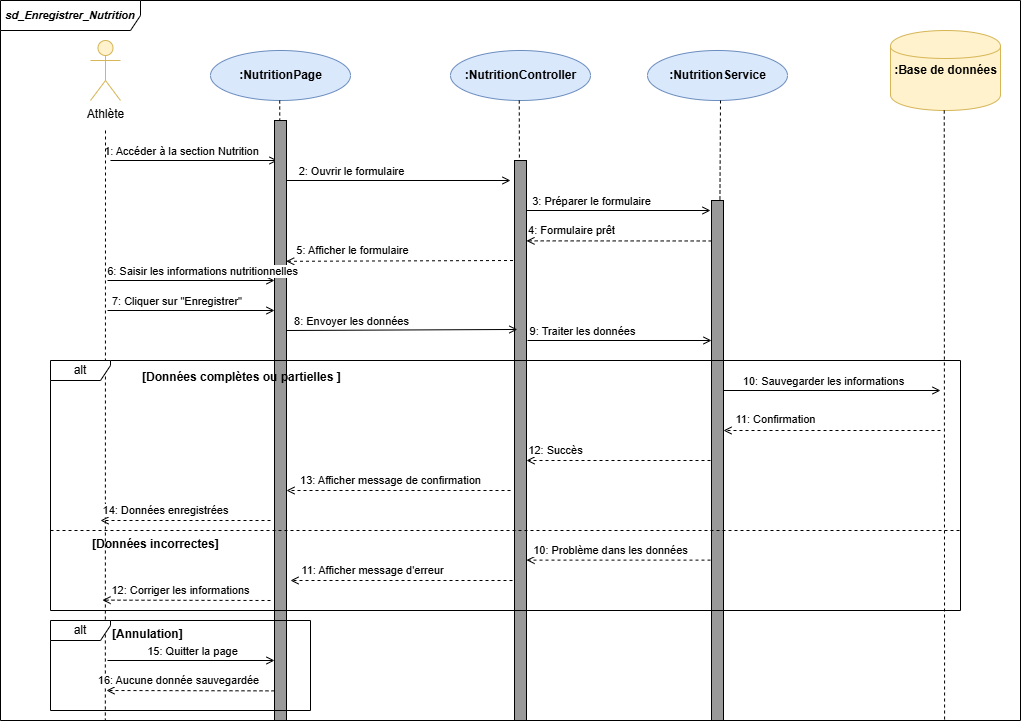
\includegraphics[width=0.9\textwidth]{images/digramme_de_sequence_de_nutrition.png}%
    }{%
        \fbox{\parbox[c][6cm][c]{0.9\textwidth}{\centering Ajouter l'image : \texttt{images/digramme\_de\_sequence\_de\_nutritions.png}}}%
    }
    \caption{Diagramme de séquence de l'enregistrement nutritionnel}
    \label{fig:sequence_nutrition_sprint2}
\end{figure}




\subsubsection*{Diagramme de séquence de la consultation des recommandations}
La figure~\ref{fig:sequence_recommandation_sprint2} illustre le scénario de consultation et de génération des recommandations personnalisées. L’athlète initie la demande depuis la page dédiée à son programme. Le système vérifie alors les informations de son profil en interrogeant la base de données. Si certaines données sont manquantes ou si un programme valide existe déjà, un message approprié est affiché. Dans le cas où une nouvelle génération est nécessaire, le système effectue les calculs métaboliques, génère les plans d’entraînement et de nutrition, puis enregistre les recommandations produites. Enfin, le programme personnalisé mis à jour est présenté à l’athlète.\begin{figure}[H]
    \centering
    \IfFileExists{images/digramme_de_sequence_recomandation.png}{%
        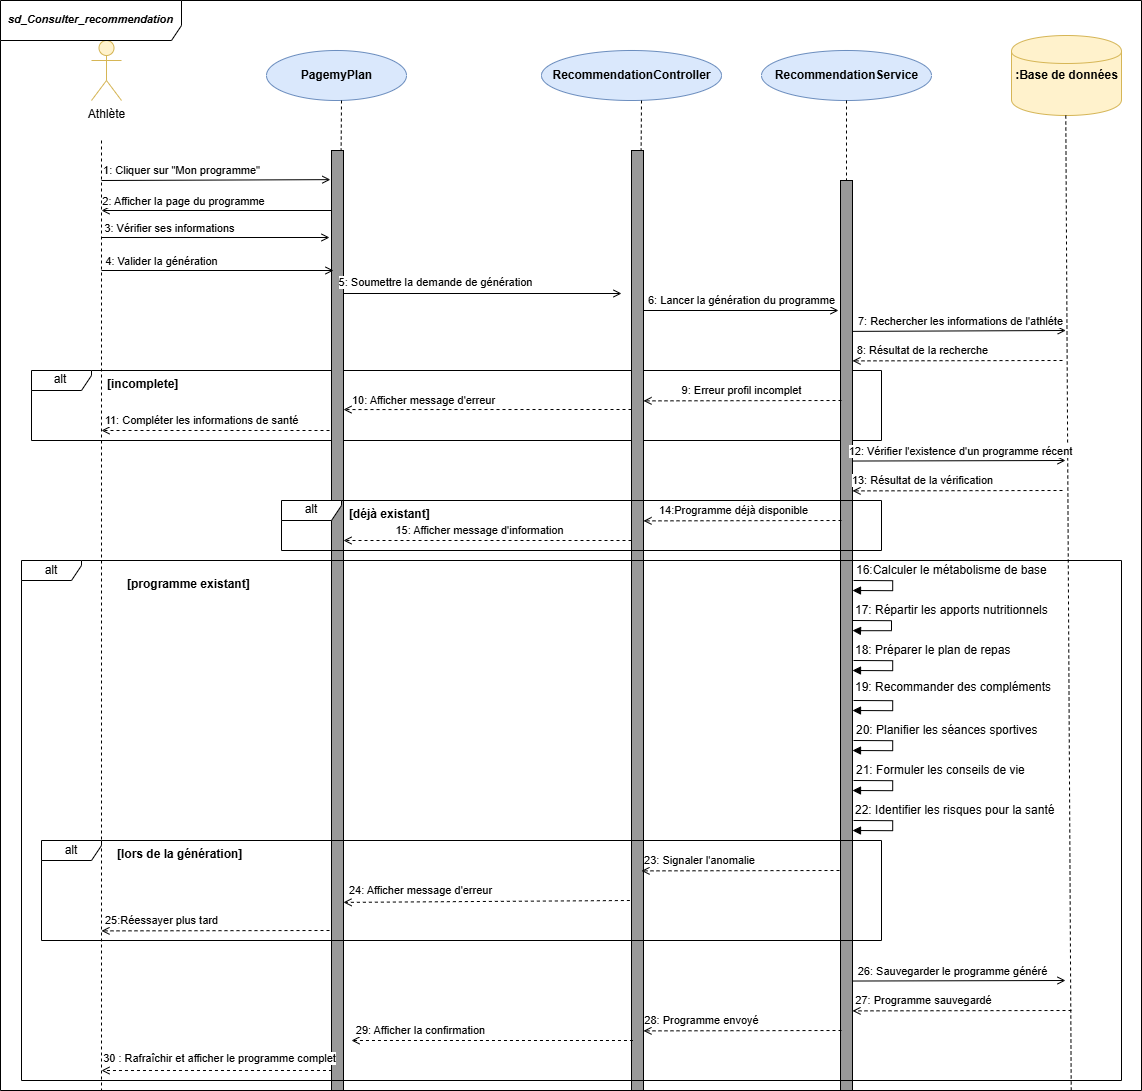
\includegraphics[width=0.9\textwidth]{images/digramme_de_sequence_recomandation.png}%
    }{%
        \fbox{\parbox[c][6cm][c]{0.9\textwidth}{\centering Ajouter l'image : \texttt{images/digramme\_de\_sequence\_recommandation.png}}}%
    }
    \caption{Diagramme de séquence de la consultation des recommandations}
    \label{fig:sequence_recommandation_sprint2}
\end{figure}


\subsection{Diagramme de classes du Sprint 2}

\begin{figure}[H]
    \centering
    \IfFileExists{images/diagramme_classes_sprint2.png}{%
        \includegraphics[width=0.95\textwidth]{images/diagramme_classes_sprint2.png}%
    }{%
        \fbox{\parbox[c][7cm][c]{0.95\textwidth}{\centering Ajouter l'image : \texttt{images/diagramme\_classes\_sprint2.png}}}%
    }
    \caption{Diagramme de classes du Sprint 2}
    \label{fig:diagramme_classes_sprint2}
\end{figure}

\section{Réalisation}

\subsection{Réalisation du suivi de l’athlète et de la gestion des plans de repas}

Cette partie présente les principales interfaces réalisées pour assurer le suivi sportif de l'athlète et la gestion des plans de repas par le nutritionniste. Les captures illustrent les écrans utilisés pour créer les plans nutritionnels, consulter leur historique, enregistrer les activités sportives et suivre l'évolution récente des séances.

\subsubsection*{Meal Plan Builder}
Le nutritionniste accède à cette vue pour créer un plan nutritionnel personnalisé pour un athlète, en définissant l'objectif calorique et en composant les repas de la journée (petit-déjeuner, déjeuner, dîner, collations) avant de sauvegarder le plan.

\begin{figure}[H]
    \centering
    \IfFileExists{images/mealplans.png}{%
        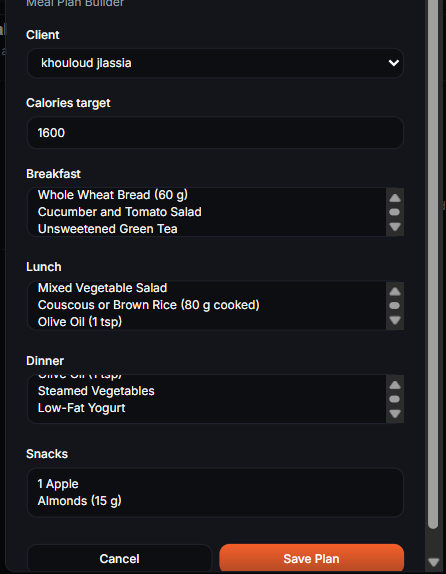
\includegraphics[width=0.95\textwidth]{images/mealplans.png}%
    }{%
        \fbox{\parbox[c][6cm][c]{0.9\textwidth}{\centering Ajouter l'image : \texttt{images/meal\_plans.png}}}%
    }
    \caption{Interface de création d'un plan nutritionnel}
    \label{fig:meal_plan_builder}
\end{figure}

\subsubsection*{Historique des Meal Plans}
Le nutritionniste consulte cette vue pour visualiser et gérer l'ensemble des plans nutritionnels créés pour ses athlètes, avec un aperçu rapide des repas de chaque journée et la possibilité de supprimer un plan existant ou d'en créer un nouveau.

\begin{figure}[H]
    \centering
    \IfFileExists{images/historiquedemealplan.png}{%
        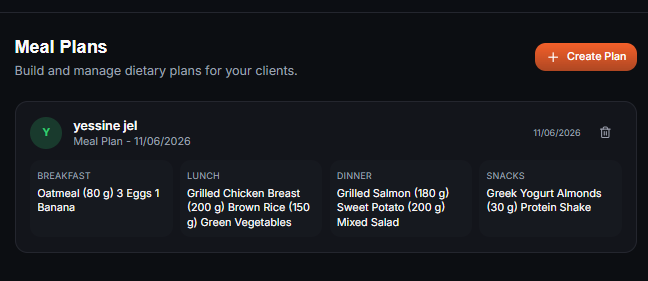
\includegraphics[width=0.95\textwidth]{images/historiquedemealplan.png}%
    }{%
        \fbox{\parbox[c][6cm][c]{0.9\textwidth}{\centering Ajouter l'image : \texttt{images/historique\_meal\_plans.png}}}%
    }
    \caption{Historique des plans nutritionnels}
    \label{fig:historique_meal_plans}
\end{figure}

\subsubsection*{Log d'activité}
L'athlète accède à cette vue pour enregistrer les activités sportives qu'il a réalisées, 
en sélectionnant le type d'activité, la durée, les calories brûlées, 
l'intensité et la date, puis en indiquant si la séance a été complétée ou manquée.
\begin{figure}[H]
    \centering
    \IfFileExists{images/logactivites.png}{%
        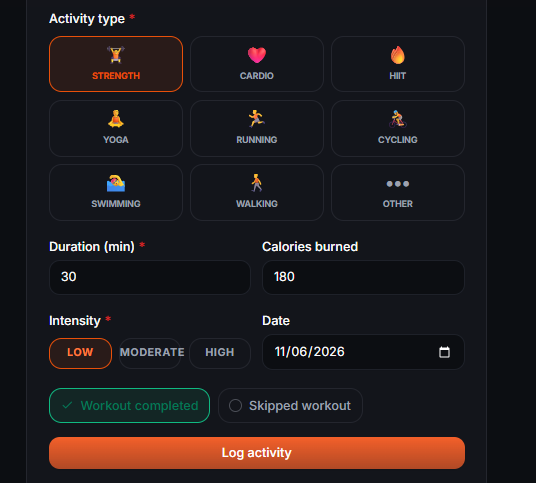
\includegraphics[width=0.95\textwidth]{images/logactivites.png}%
    }{%
        \fbox{\parbox[c][6cm][c]{0.9\textwidth}{\centering Ajouter l'image : \texttt{images/log\_activites.png}}}%
    }
    \caption{Interface d'enregistrement d'une activité sportive}
    \label{fig:log_activite}
\end{figure}

\subsubsection*{Activité récente}
L'athlète consulte cette vue pour suivre l'historique des activités sportives 
qu'il a enregistrées, avec un graphique illustrant l'évolution de la durée et des 
calories brûlées sur une période donnée, ainsi qu'un récapitulatif détaillé de chaque séance réalisée.

\begin{figure}[H]
    \centering
    \IfFileExists{images/recentactivity.png}{%
        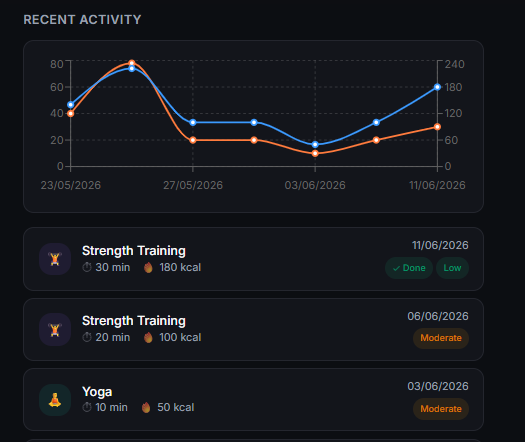
\includegraphics[width=0.95\textwidth]{images/recentactivity.png}%
    }{%
        \fbox{\parbox[c][6cm][c]{0.9\textwidth}{\centering Ajouter l'image : \texttt{images/recentactivity.png}}}%
    }
    \caption{Suivi des activités récentes de l'athlète}
    \label{fig:recentactivity}
\end{figure}


\subsection{Modèles d’intelligence artificielle}

\subsection{Système de recommandations basé sur des règles (Rules-Based)}

\subsection{Chatbot IA}

\section{Conclusion}

Au cours de ce sprint, nous avons enrichi la plateforme UFitPal avec des fonctionnalités orientées vers le suivi personnalisé de l'athlète. Ces fonctionnalités permettent de centraliser les données sportives et nutritionnelles, de consulter les plans proposés par les professionnels et d'exploiter les premiers résultats issus des modèles d'intelligence artificielle. Le chapitre suivant pourra ainsi approfondir les fonctionnalités avancées et les améliorations apportées à l'expérience utilisateur.

\chapter*{Conclusion générale}
\addcontentsline{toc}{chapter}{Conclusion générale}

Notre stage au sein de HOLMENA Company for Digital Solutions fut une expérience riche en apprentissages et en réalisations. Malgré les obstacles rencontrés, notamment lors de l'intégration des modules d'intelligence artificielle et de la mise en place de l'architecture technique, nous avons fait preuve de persévérance et mené à bien le projet qui nous était confié. Cette immersion professionnelle nous a permis de développer nos compétences et d'apprécier la valeur du travail en équipe au sein d'un environnement dynamique et stimulant.

Notre projet de conception et de développement de la plateforme intelligente de fitness et de nutrition « UFitPal » représente une étape significative. À travers notre étude, nous avons identifié la nécessité d'une telle plateforme pour offrir aux athlètes un suivi personnalisé et adapté à leurs besoins, tout en facilitant la collaboration avec les coachs sportifs et les nutritionnistes et en intégrant des solutions basées sur l'intelligence artificielle.

Nous avons suivi rigoureusement chacune des étapes de ce projet, de l'étude de l'existant à la conception puis à la réalisation des différents sprints de l'application. En définissant précisément les objectifs, en planifiant avec soin les tâches suivant la méthodologie Scrum et en prenant en compte les besoins des divers acteurs, nous avons jeté les bases solides d'une plateforme potentiellement florissante et porteuse d'effets concrets.

Ce stage nous a également donné l'opportunité d'explorer et de maîtriser de nouvelles technologies modernes, telles que Next.js, NestJS, TypeScript, PostgreSQL et Python, et d'en acquérir une maîtrise précieuse.

Le projet peut être amélioré en intégrant de nouvelles fonctionnalités telles que :

\begin{itemize}[label=\ding{226}]
    \item Rendre notre application disponible en version mobile native sur iOS et Android.
    \item Intégrer des dispositifs portables connectés (\textit{Wearable Devices}), tels que des montres intelligentes et des bracelets de fitness, permettant une collecte automatique et continue des données biométriques de l'athlète.
    \item Mettre en place un système de suivi fitness basé sur l'IoT, permettant une synchronisation en temps réel des données sportives entre les capteurs connectés et la plateforme UFitPal.
\end{itemize}

\end{document}
 